%!TEX root = ../thesis.tex
%*******************************************************************************
%****************************** Second Chapter *********************************
%*******************************************************************************

\chapter{Score-based Pullback Riemannian Geometry}\label{Chapter:Pullback-riemannian-geometry}

\ifpdf
    \graphicspath{{Chapter5/Figs/Raster/}{Chapter5/Figs/PDF/}{Chapter5/Figs/}}
\else
    \graphicspath{{Chapter5/Figs/Vector/}{Chapter5/Figs/}}
\fi

Data-driven Riemannian geometry has emerged as a powerful tool for interpretable representation learning, offering improved efficiency in downstream tasks. Moving forward, it is crucial to balance cheap manifold mappings with efficient training algorithms. In this work, we integrate concepts from pullback Riemannian geometry and generative models to propose a framework for data-driven Riemannian geometry that is scalable in both geometry and learning: score-based pullback Riemannian geometry. Focusing on unimodal distributions as a first step, we propose a score-based Riemannian structure with closed-form geodesics that pass through the data probability density. With this structure, we construct a Riemannian autoencoder (RAE) with error bounds for discovering the correct data manifold dimension. This framework can naturally be used with anisotropic normalizing flows by adopting isometry regularization during training. Through numerical experiments on diverse datasets, including image data, we demonstrate that the proposed framework produces high-quality geodesics passing through the data support, reliably estimates the intrinsic dimension of the data manifold, and provides a global chart of the manifold. To the best of our knowledge, this is the first scalable framework for extracting the complete geometry of the data manifold.

\section{Introduction}

Data often reside near low-dimensional non-linear manifolds as illustrated in Figure~\ref{fig:learned_charts}. This manifold assumption \cite{fefferman2016testing} has been popular since the early work on non-linear dimension reduction \cite{belkin2001laplacian,coifman2006diffusion,roweis2000nonlinear,sammon1969nonlinear,tenenbaum2000global}. Learning this non-linear structure, or representation learning, from data has proven to be highly successful \cite{demers1992non,kingma2013auto} and continues to be a recurring theme in modern machine learning approaches and downstream applications \cite{chow2022predicting,gomari2022variational,ternes2022multi,vahdat2020nvae,zhong2021cryodrgn}. 

Recent advances in data-driven Riemannian geometry have demonstrated its suitability for learning representations.
In this context, these representations are elements residing in a learned geodesic subspace of the data space, governed by a non-trivial Riemannian structure\footnote{rather than the standard $\ell^2$-inner product} across the entire ambient space \cite{arvanitidis2016locally,diepeveen2024pulling,hauberg2012geometric,peltonen2004improved,Scarvelis2023,sorrenson2024learningdistancesdatanormalizing,sun2024geometryaware}. 
Among these contributions, it is worth highlighting that \cite{sorrenson2024learningdistancesdatanormalizing} are the first and only ones so far to use information from the full data distribution obtained though generative models \cite{dinh2017density,song2020score}, even though this seems a natural approach given recent studies such as \cite{NEURIPS2022_4f918fa3,tempczyk2022lidl,sakamoto2024the,pmlr-v235-stanczuk24a}. A possible explanation for the limited use of generative models in constructing Riemannian geometry could lie in challenges regarding \emph{scalability of the manifold mappings}. Indeed, even though the generative models can be trained efficiently, \cite{sorrenson2024learningdistancesdatanormalizing} also mention themselves that it can be numerically challenging to work with their induced Riemannian geometry.

\begin{figure}[t]
    \centering
    \begin{subfigure}[b]{0.32\textwidth}
        \centering
        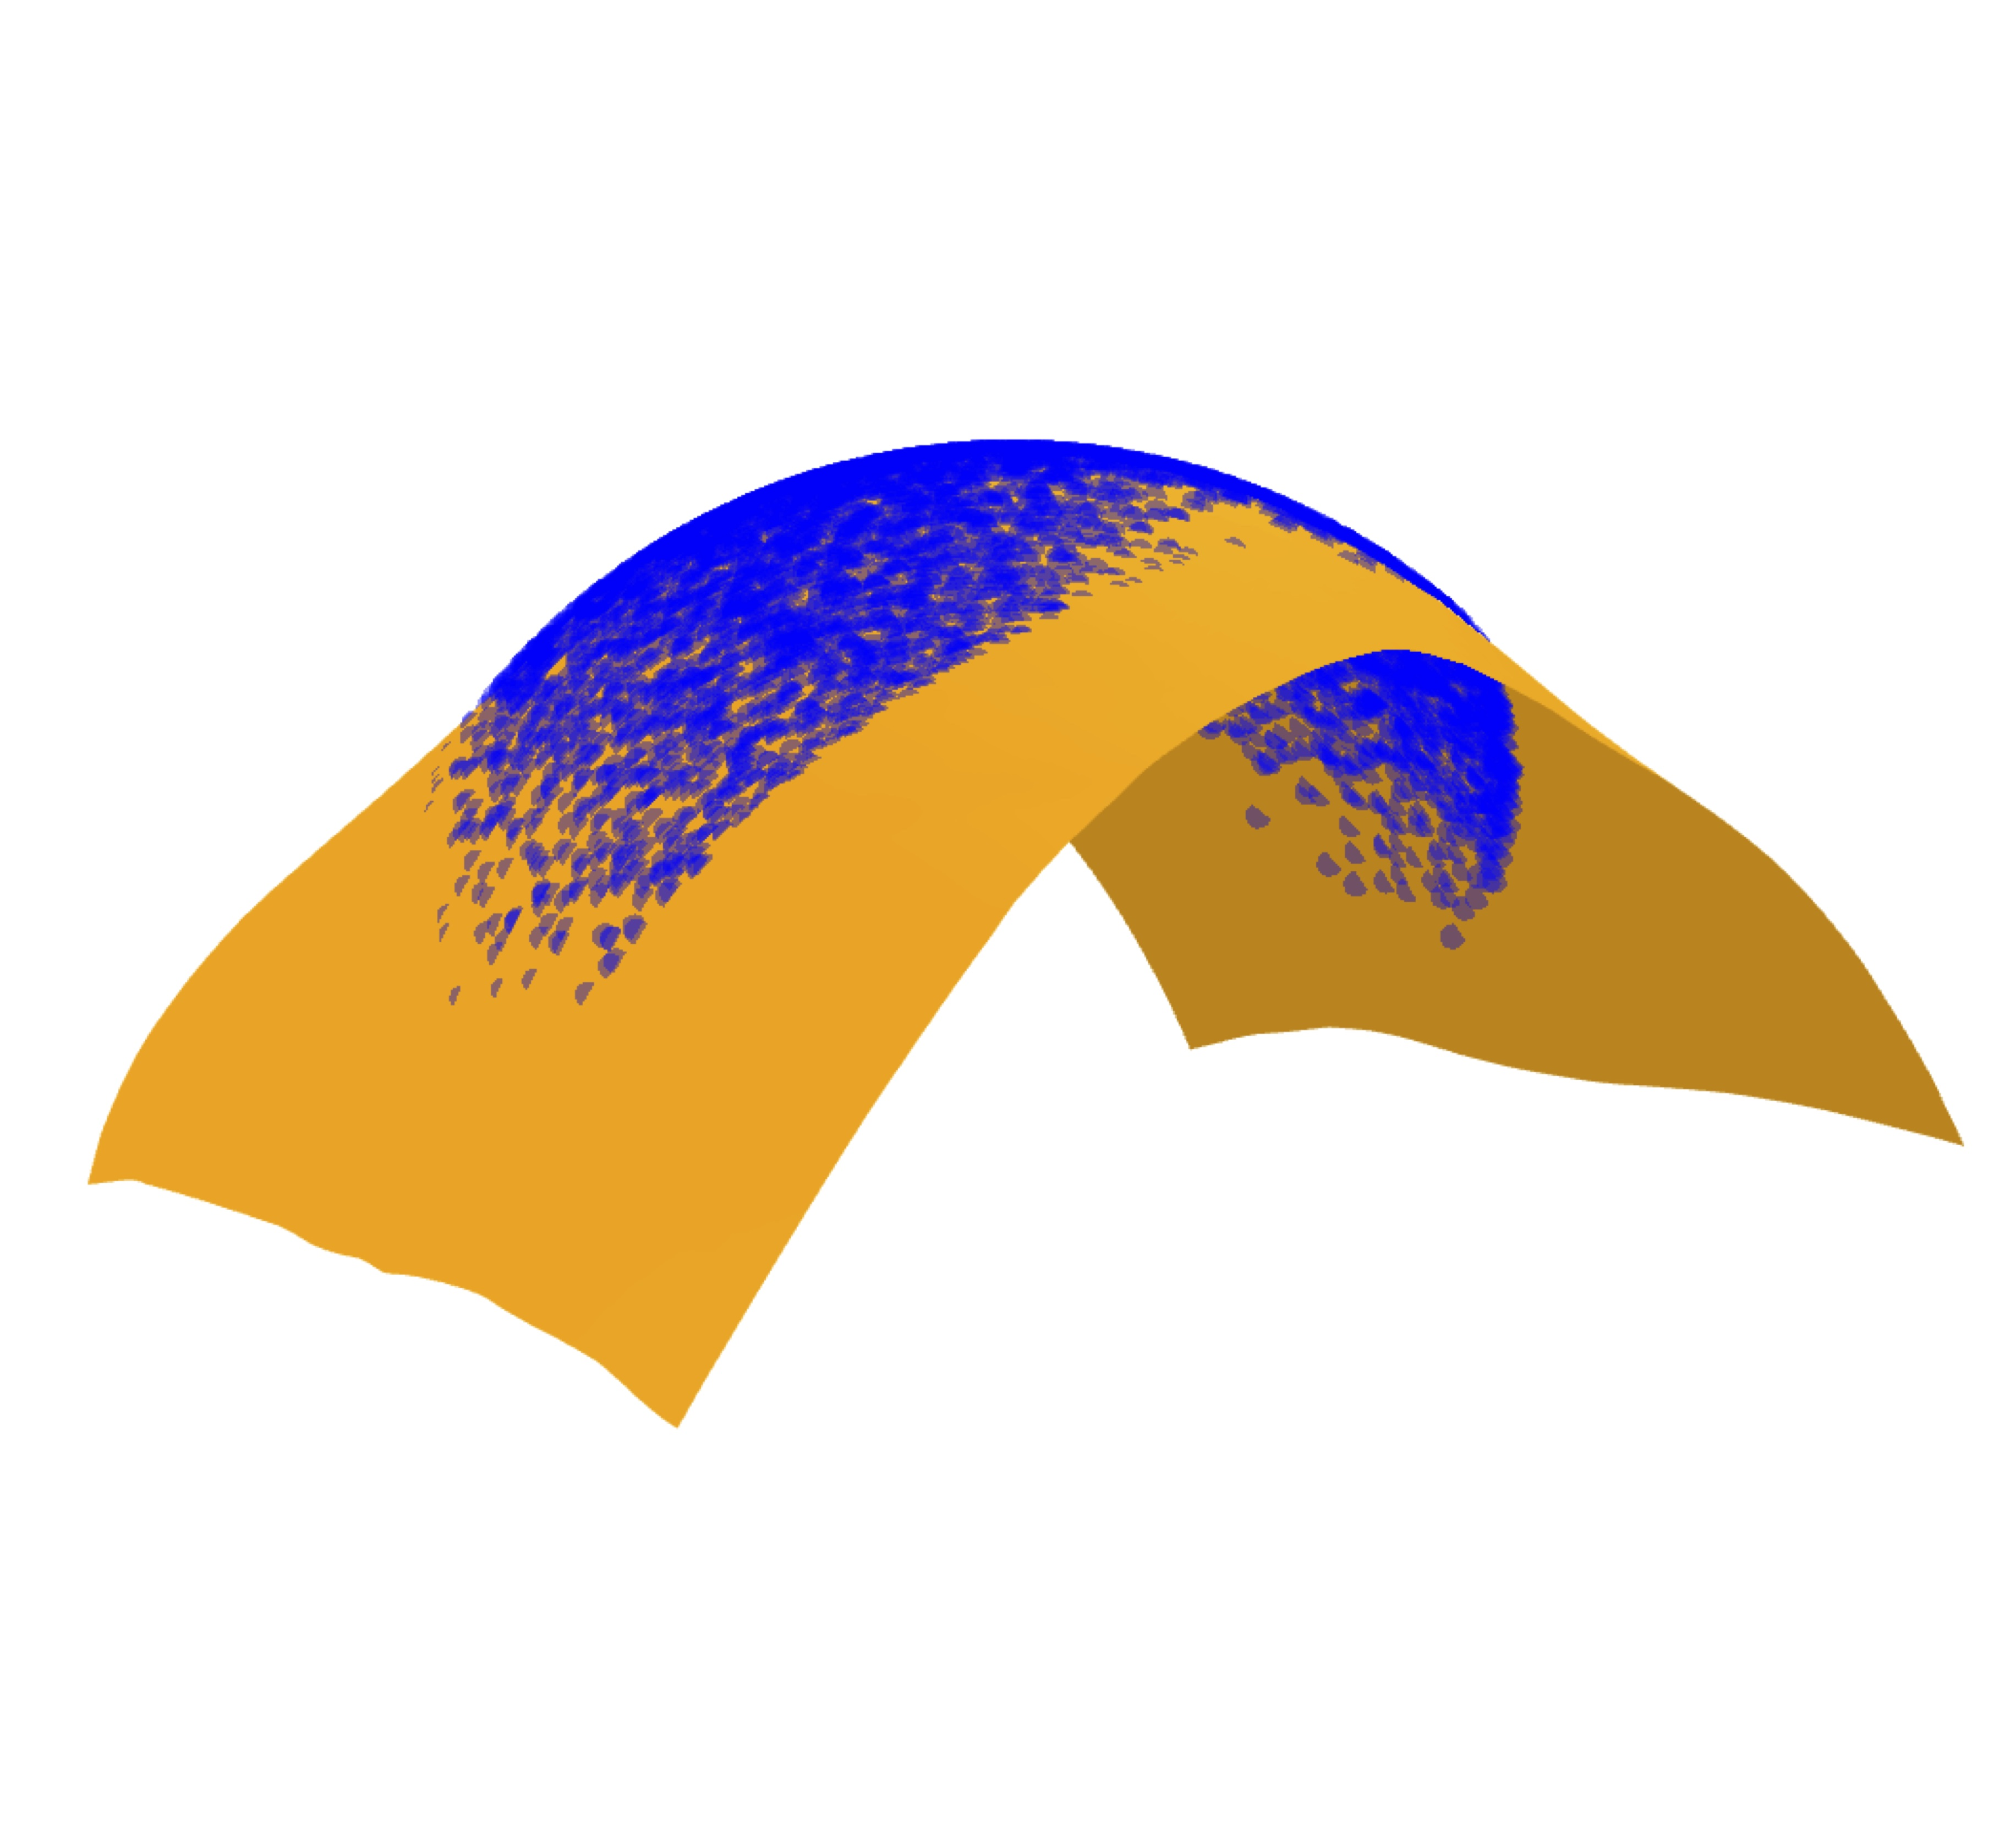
\includegraphics[width=\textwidth]{Chapter5/results/visualisations/RAE/projections/hemisphere_2_3/riemannian_autoencoder.jpg}
        \caption{Hemisphere (2,3)}
    \end{subfigure}
    \hfill
    \begin{subfigure}[b]{0.32\textwidth}
        \centering
        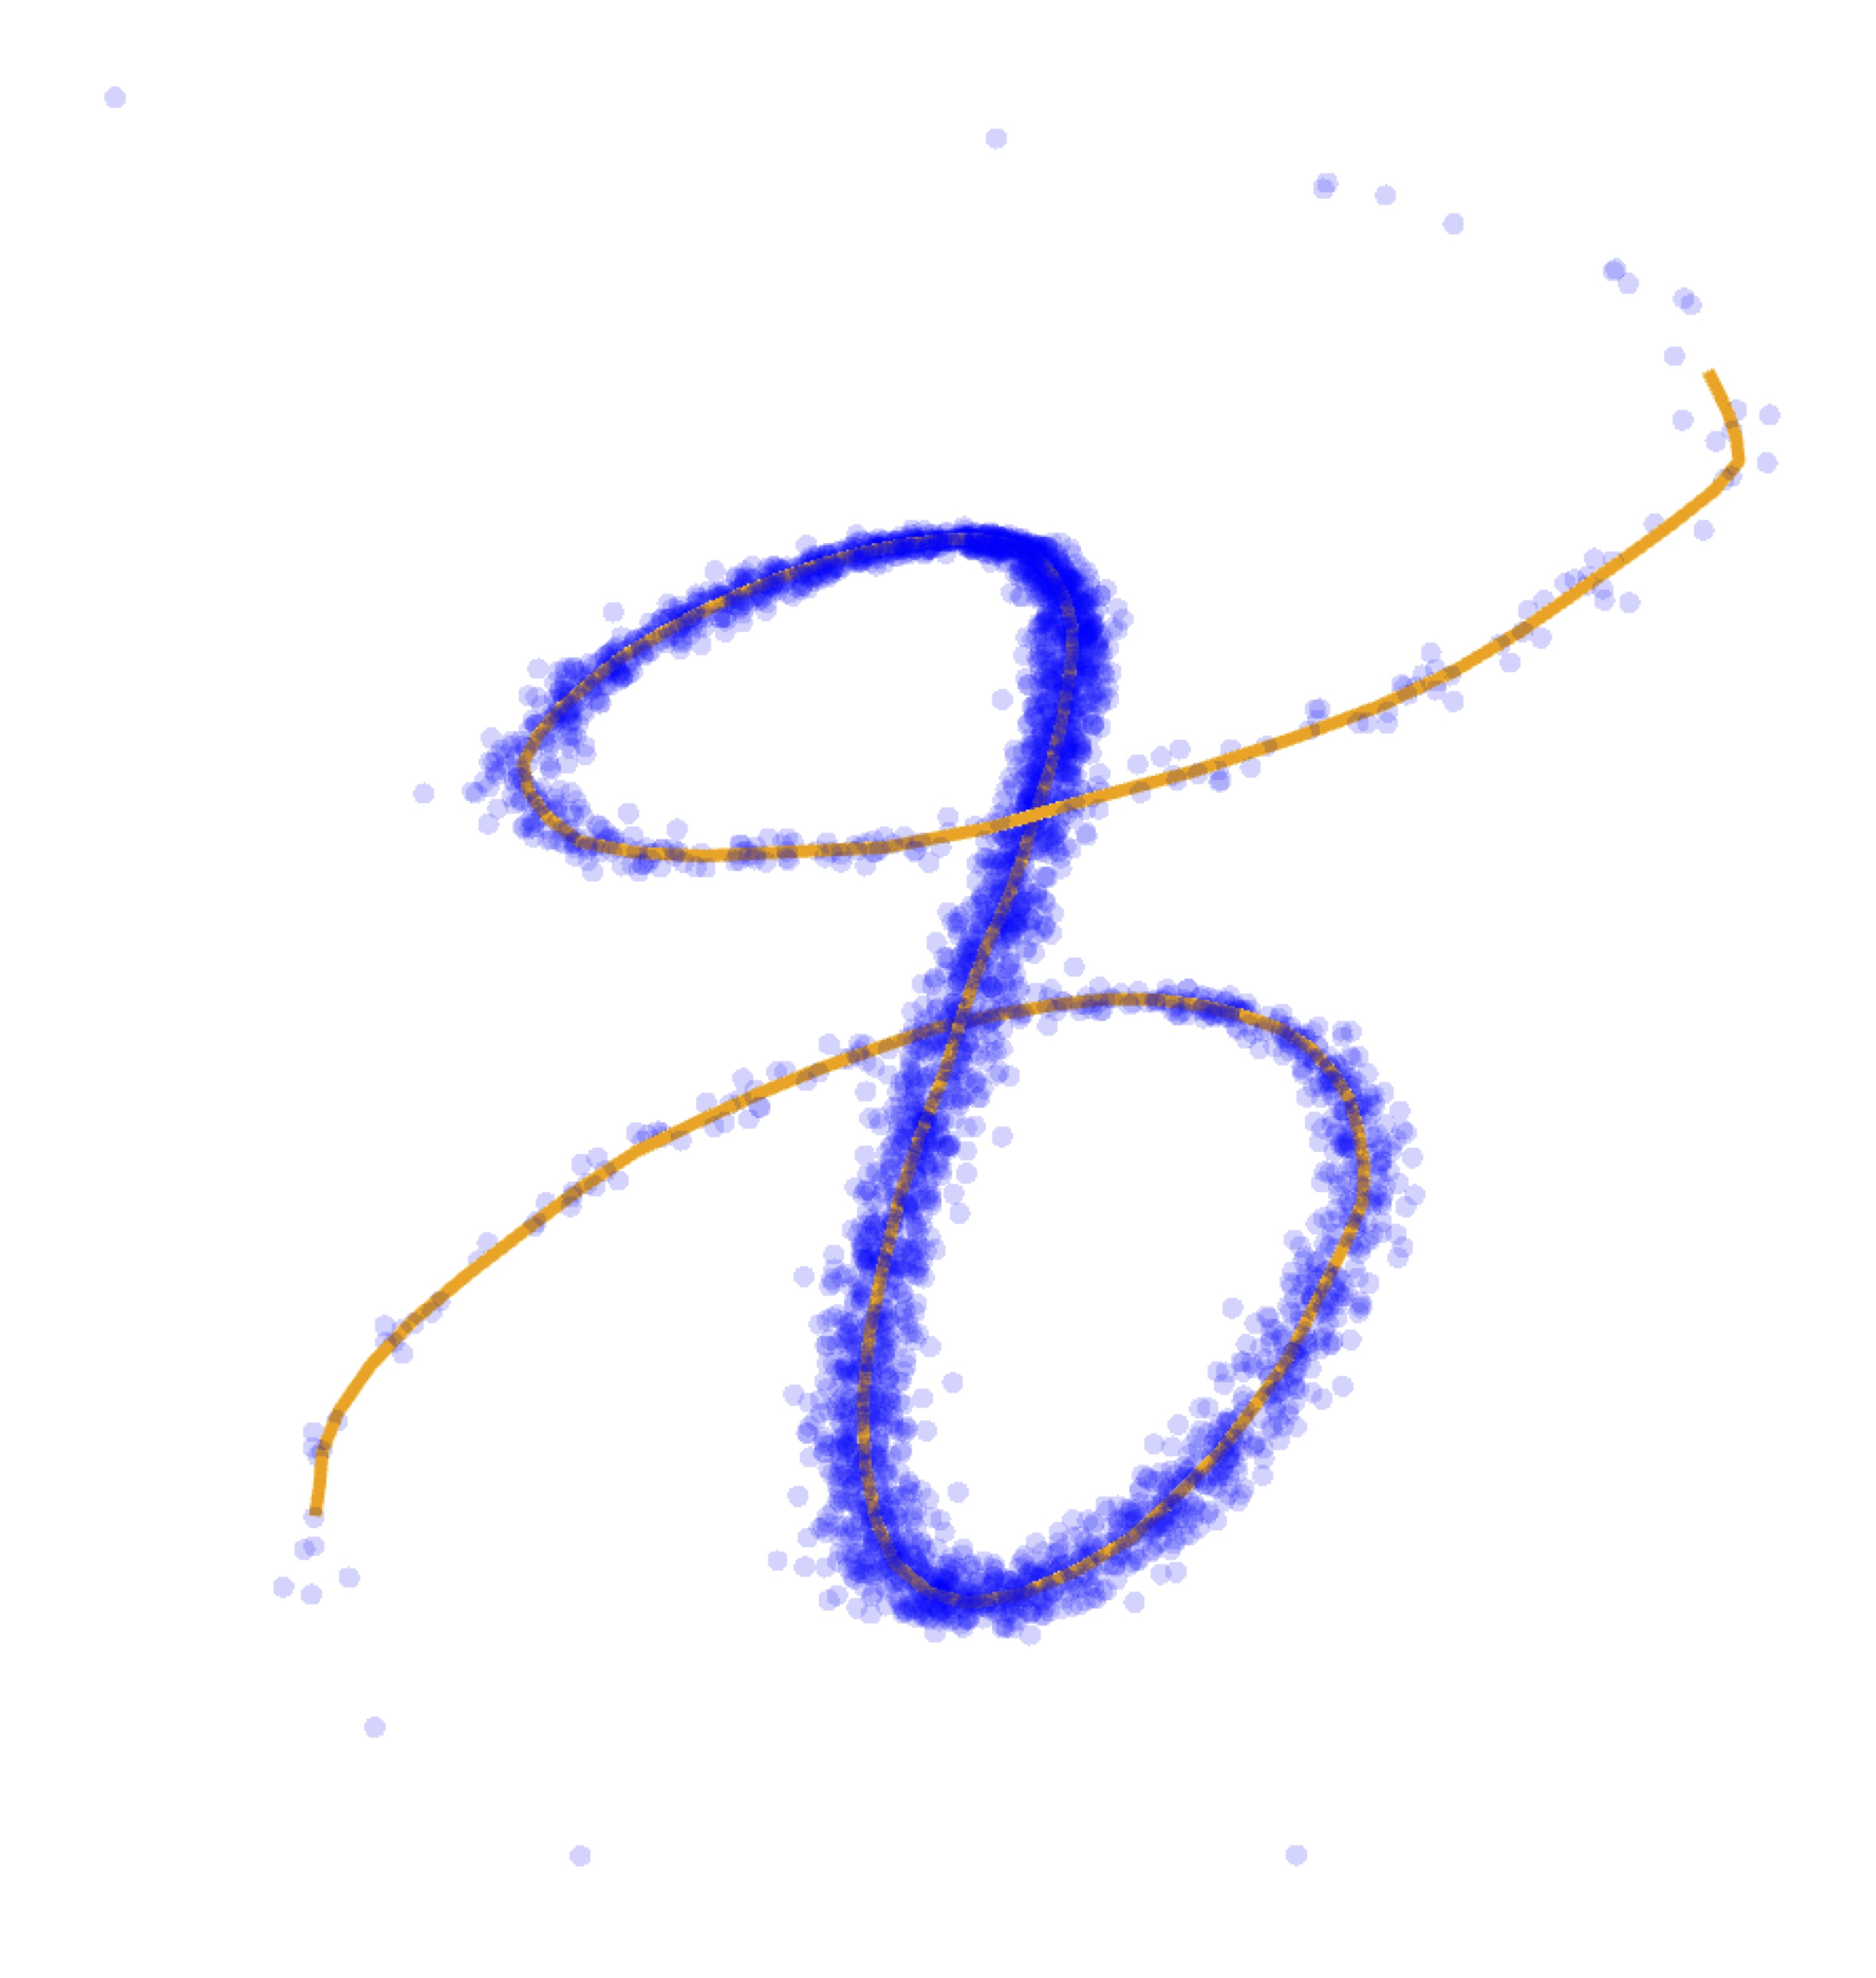
\includegraphics[width=\textwidth]{Chapter5/results/visualisations/RAE/projections/sinusoid_1_3/riemannian_autoencoder.jpg}
        \caption{Sinusoid (1,3)}
    \end{subfigure}
    \hfill
    \begin{subfigure}[b]{0.32\textwidth}
        \centering
        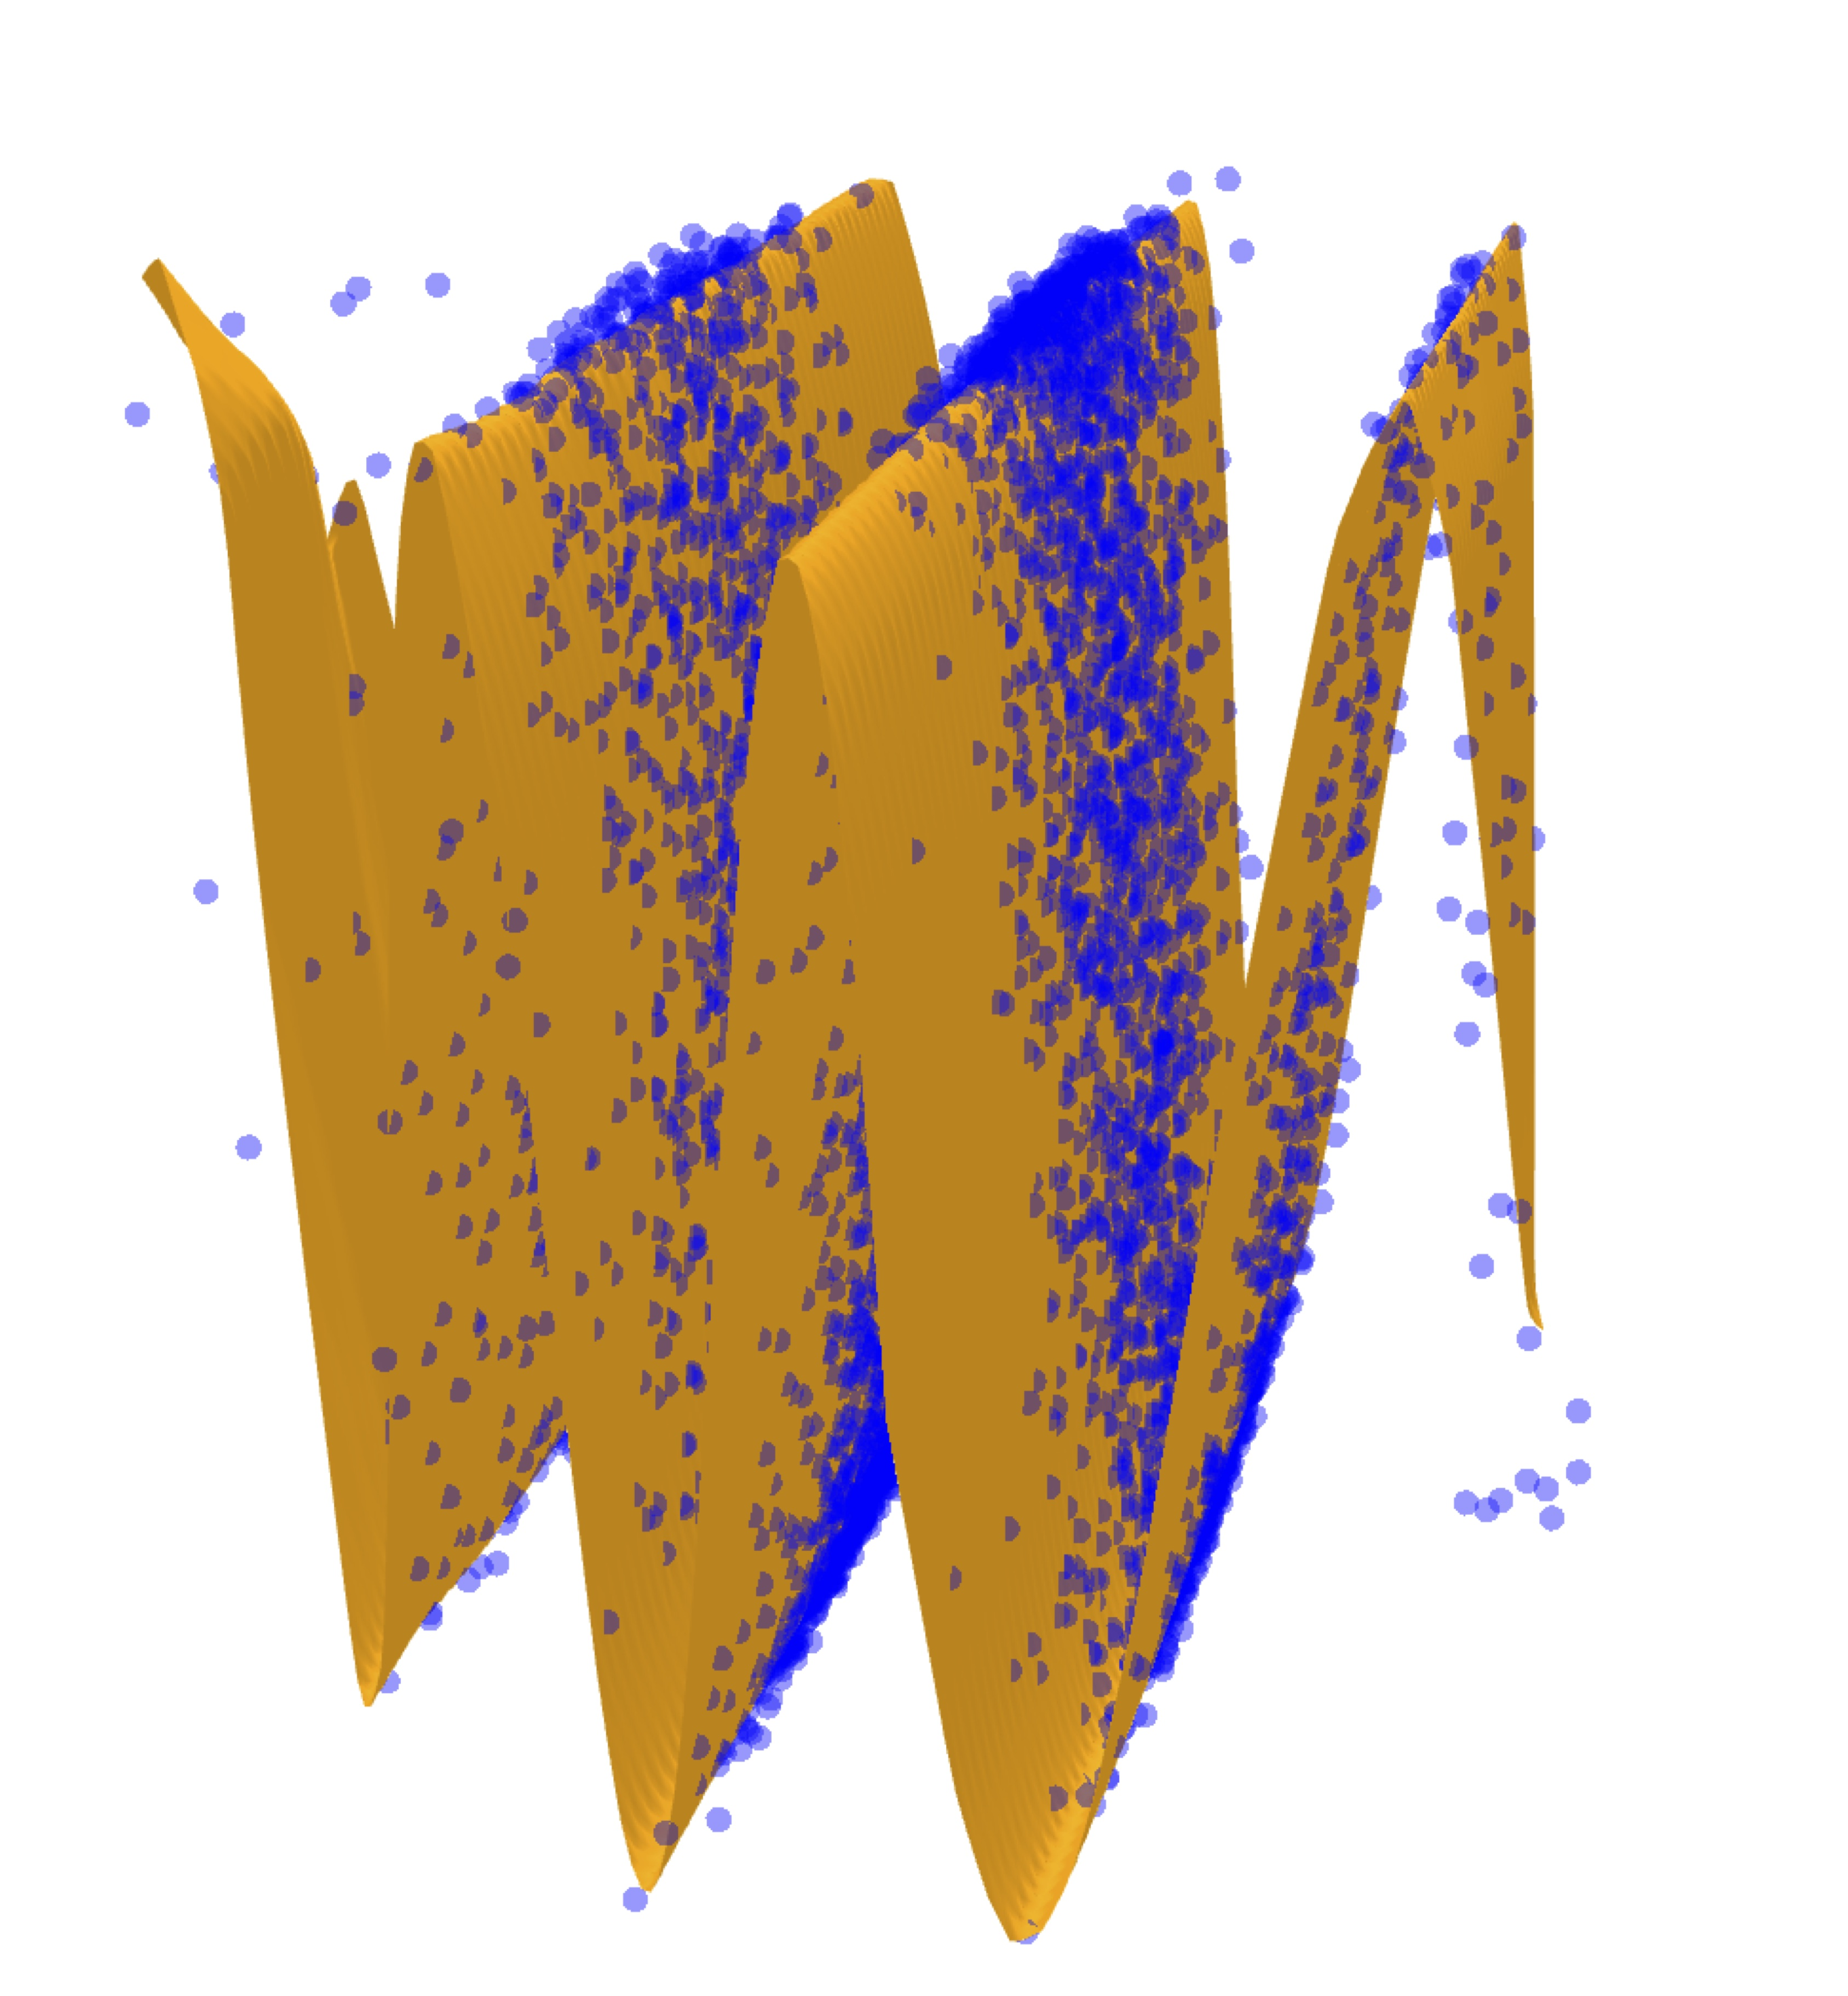
\includegraphics[width=\textwidth]{Chapter5/results/visualisations/RAE/projections/sinusoid_2_3/riemannian_autoencoder.jpg}
        \caption{Sinusoid (2,3)}
    \end{subfigure}

    \caption{
        Approximate data manifolds learned by the Riemannian autoencoder generated by score-based pullback Riemannian geometry for three datasets. The orange surfaces represent the manifolds learned by the model, while the blue points correspond to the training data. Each manifold provides a convincing low-dimensional representation of the data, isometric to its respective latent space.
    }
    \label{fig:learned_charts}
\end{figure}

If the manifold mapping scalability challenges were to be overcome, the combined power of Riemannian geometry and state of the art generative modelling could have profound implications on how to handle data in general. 
Indeed, beyond typical data analysis tasks such as computing distances, means, and interpolations/extrapolations of data points,

a data-driven Riemannian structure also offers greater potential for representation learning and downstream applications. For instance, many advanced data processing methods, from Principal Component Analysis (PCA) to score and flow-matching, have Riemannian counterparts (\cite{diepeveen2023curvature,fletcher2004principal} and \cite{chen2023riemannian,huang2022riemannian}) that have proven beneficial by improving upon full black box methods in terms of interpretability \cite{diepeveen2024pulling} or Euclidean counterparts in terms of efficiency \cite{kapusniak2024metricflowmatchingsmooth,de2024pullback}. 

Here it is worth highlighting that scalability of manifold mappings was completely circumvented by \cite{diepeveen2024pulling} and \cite{de2024pullback} by using pullback geometry. 
However, here learning a suitable (and stable) pullback geometry suffers from challenges regarding \emph{scalability of the training algorithm}, contrary to the approach by \cite{sorrenson2024learningdistancesdatanormalizing}.

Motivated by the above, this work aims to address the following question: How to strike a good balance between scalability of training a data-driven Riemannian structure and of evaluating its corresponding manifold mappings?

\subsection{Contributions}
In this paper, we take first steps towards striking such a balance and propose a score-based pullback Riemannian metric assuming a relatively simple but generally applicable family of probability densities, which we show to result in both scalable manifold mappings and scalable learning algorithms. We emphasize that we do not directly aim to find the perfect balance between the two types of scalability. Instead we start from a setting which has many nice properties, but will allow for generalization to multimodal densities, which we reserve for future work.

Specifically, we consider a family of unimodal probability densities whose negative log-likelihoods are compositions of strongly convex functions and diffeomorphisms. As this work is an attempt to bridge between the geometric data analysis community and the generative modeling community, we break down the contributions in two ways.
Theoretically,
\begin{itemize}
    % \item \new 
    % We show that in analogy with the fisher information metric, considering the symmetrized KL divergence between denoising posteriors naturally results in a pullback - based metric.
    \item We propose a score-based pullback Riemannian metric such that manifold mappings respect the data distribution.
    \item We demonstrate that this density-based Riemannian structure naturally leads to a Riemannian autoencoder\footnote{in the sense of \cite{diepeveen2024pulling}} and provide error bounds on the expected reconstruction error, which allows for approximation of the data manifold as illustrated in Figure~\ref{fig:learned_charts}.
    \item We introduce a learning scheme based on adaptations of normalizing flows to find the density to be integrated into the Riemannian framework, which is tested on several synthetic data sets. 
\end{itemize}
Practically, this work showcases how two simple adaptations to the normalizing flows framework enable data-driven Riemannian geometry. This significantly expands the potential for downstream applications compared to the unadapted framework.


\subsection{Outline}

After introducing notation in Section~\ref{sec:notation}, Section~\ref{sec:unimodal-riemannian geometry} considers a family of probability distributions, from which we obtain suitable geometry, and Section~\ref{sec:rae} showcases how one can subsequently construct Riemannian Autoencoders with theoretical guarantees. From these observation, Section~\ref{sec:adapting-normalising-flows} discusses the natural limitations of standard normalizing flows and how to change the parametrisation and training for downstream application in a Riemannian geometric setting. Section~\ref{sec:numerics} showcases several use cases of data-driven Riemannian structure on several data sets. Finally, we summarize our findings in Section~\ref{sec:conclusions}.


\section{Notation}
\label{sec:notation}

% \subsection{Differential Geometry}
Here we present some basic notations from differential and Riemannian geometry, see \cite{boothby2003introduction,carmo1992riemannian,lee2013smooth,sakai1996riemannian} for details. 
% \dn{What does this sentence mean exactly? Maybe instead say something like "Here we present some basics and notation from differential and Riemannian geometry, see \cite{}... for more details." ?} \wdp{fixed}


\textit{Smooth Manifolds and Tangent Spaces}. Let $\manifold$ be a smooth manifold. We write $C^\infty(\manifold)$ for the space of smooth functions over $\manifold$. The \emph{tangent space} at $\mPoint \in \manifold$, which is defined as the space of all \emph{derivations} at $\mPoint$, is denoted by $\tangent_\mPoint \manifold$ and for \emph{tangent vectors} we write $\tangentVector_\mPoint \in \tangent_\mPoint \manifold$. For the \emph{tangent bundle} we write $\tangent\manifold$ and smooth vector fields, which are defined as \emph{smooth sections} of the tangent bundle, are written as $\vectorfield(\manifold) \subset \tangent\manifold$.
% Furthermore, additional structure on manifolds and derived notions thereof are typically defined through tensor fields of the form $T~:~\vectorfield(\manifold)^n \to \vectorfield(\manifold)^m$ or $T~:~\vectorfield(\manifold)^n \to C^\infty(\manifold)$. A tensor field can -- by definition of being $C^\infty(\manifold)$-modules -- be restricted to a tangent space at each point $\mPoint \in \manifold$, for which we use the notation $T_{\mPoint}: \tangent_\mPoint \manifold^n \to \tangent_\mPoint \manifold^m$ or $T_{\mPoint}: \tangent_\mPoint \manifold^n \to \Real$. 

\textit{Riemannian Manifolds}. A smooth manifold $\manifold$ becomes a \emph{Riemannian manifold} if it is equipped with a smoothly varying \emph{metric tensor field} $(\,\cdot\,, \,\cdot\,) \colon \vectorfield(\manifold) \times \vectorfield(\manifold) \to C^\infty(\manifold)$. This tensor field induces a \emph{(Riemannian) metric} $\distance_{\manifold} \colon \manifold\times\manifold\to\Real$. The metric tensor can also be used to construct a unique affine connection, the \emph{Levi-Civita connection}, that is denoted by $\nabla_{(\,\cdot\,)}(\,\cdot\,) : \vectorfield(\manifold) \times \vectorfield(\manifold) \to \vectorfield(\manifold)$. 
This connection is in turn the cornerstone of a myriad of manifold mappings.

\textit{Geodesic.} One is the notion of a \emph{geodesic}, which for two points $\mPoint,\mPointB \in \manifold$ is defined as a curve $\geodesic_{\mPoint,\mPointB} \colon [0,1] \to \manifold$ with minimal length that connects $\mPoint$ with $\mPointB$. Another closely related notion to geodesics is the curve $t \mapsto \geodesic_{\mPoint,\tangentVector_\mPoint}(t)$  for a geodesic starting from $\mPoint\in\manifold$ with velocity $\dot{\geodesic}_{\mPoint,\tangentVector_\mPoint} (0) = \tangentVector_\mPoint \in \tangent_\mPoint\manifold$. 

\textit{Exponential Map}. This can be used to define the \emph{exponential map} $\exp_\mPoint \colon \mathcal{D}_\mPoint \to \manifold$ as \(\exp_\mPoint(\tangentVector_\mPoint) := \geodesic_{\mPoint,\tangentVector_\mPoint}(1),\) where \(\mathcal{D}_\mPoint \subset \tangent_\mPoint \manifold\) is the set on which \(\geodesic_{\mPoint,\tangentVector_\mPoint}(1)\) is defined.
% The manifold $\manifold$ is said to be \emph{(geodesically) complete} whenever $\mathcal{D}_\mPoint = \mathcal{T}_{\mPoint}\manifold$ for all $\mPoint \in \manifold$.

\textit{Logarithmic Map}. Furthermore, the \emph{logarithmic map} $\log_\mPoint \colon \exp(\mathcal{D}'_\mPoint ) \to \mathcal{D}'_\mPoint$ is defined as the inverse of $\exp_\mPoint$, so it is well-defined on  $\mathcal{D}'_{\mPoint} \subset \mathcal{D}_{\mPoint}$ where $\exp_\mPoint$ is a diffeomorphism. 


\textit{Pullback metrics}. Finally, if $(\manifold, (\cdot,\cdot))$ is a $\dimInd$-dimensional Riemannian manifold, $\manifoldB$ is a $\dimInd$-dimensional smooth manifold and $\diffeoB:\manifoldB \to \manifold$ is a diffeomorphism, the \emph{pullback metric}
\begin{equation}
    (\tangentVector, \tangentVectorB)^\diffeoB := (D_{(\cdot)}\diffeoB[\tangentVector_{(\cdot)}], D_{(\cdot)}\diffeoB[\tangentVectorB_{(\cdot)}])_{\diffeoB(\cdot)},
    \label{eq:pull-back-metric}
\end{equation}
where $D_{\mPoint}\diffeoB: \tangent_\mPoint \manifoldB \to \tangent_{\diffeoB(\mPoint)} \manifold$ denotes the differential of $\diffeoB$,
% or 
% \begin{equation}
%     (\tangentVector, \tangentVectorB)^\diffeoB := (\diffeoB_*[\tangentVector], \diffeoB_*[\tangentVectorB])
%     \label{eq:pull-back-metric}
% \end{equation}
defines a Riemannian structure on $\manifoldB$, which we denote by $(\manifoldB, (\cdot,\cdot)^\diffeoB)$. 
Pullback metrics literally pull back all geometric information from the Riemannian structure on $\manifold$. 
% In particular, closed-form manifold mappings on $(\manifold, (\cdot,\cdot))$ yield under mild assumptions closed-form manifold mappings on $(\manifoldB, (\cdot,\cdot)^\diffeoB)$.
Throughout the rest of the paper pullback mappings will be denoted similarly to Equation~\ref{eq:pull-back-metric} with the diffeomorphism $\diffeoB$ as a superscript, i.e., we write $\distance^\diffeoB_{\manifoldB}(\mPoint, \mPointB)$, $\geodesic^\diffeoB_{\mPoint, \mPointB}$, $\exp^\diffeoB_\mPoint (\tangentVector_\mPoint)$ and $\log^\diffeoB_{\mPoint} \mPointB$ 
% and $\mathcal{P}^\diffeoB_{\mPointB \leftarrow \mPoint} \tangentVector_\mPoint$ 
for $\mPoint,\mPointB \in \manifoldB$ and $\tangentVector_\mPoint \in \tangent_\mPoint \manifoldB$. 


\section{Riemannian geometry from unimodal probability densities}
\label{sec:unimodal-riemannian geometry}

% \todo{I propose to first define the metric in its most general form from the score, then followed by this section - want to keep this as general as we can for as long as we can.}
We remind the reader that the ultimate goal of data-driven Riemannian geometry on $\Real^\dimInd$ is to construct a Riemannian structure such that geodesics always pass through the support of data probability densities. In this section we will focus on constructing Riemannian geometry that does just that from unimodal densities $\density:\Real^\dimInd\to \Real$ of the form
\begin{equation}
    \density(\Vector) \propto e^{- \stroco(\diffeo(\Vector))},
    \label{eq:stroco-diffeo-density}
\end{equation}
where $\stroco:\Real^\dimInd\to\Real$ is a smooth strongly convex function and $\diffeo:\Real^\dimInd\to\Real^\dimInd$ is a diffeomorphism.
% , e.g., such as the density in \ref{fig:toy-example}\footnote{Here, $\stroco(\Vector) := 2 \Vector_1^2 + \frac{1}{8}\Vector_2^2$ and $\diffeo(\Vector):= (\Vector_1 - \frac{1}{9} \Vector_2^2, \Vector_2)$.}. 
In particular, we will consider pullback Riemannian structures of the form\footnote{Note that $\nabla \stroco \circ \diffeo$ should be read as $(\nabla \stroco) \circ \diffeo$.}
\begin{equation}
    (\tangentVector, \tangentVectorB)^{\nabla \stroco \circ \diffeo}_{\Vector} := (D_{\Vector} \nabla \stroco \circ \diffeo[\tangentVector], D_{\Vector} \nabla \stroco \circ \diffeo[\tangentVectorB])_2.
    \label{eq:stroco-diffeo-pullback}
\end{equation}
For proofs of the results below and those of more general statements we refer the reader to Appendix~\ref{app:proof-of-basic-setup}.


The following result, which is a direct application of \cite[Prop.~2.1]{diepeveen2024pulling}, gives us closed-form expressions of several important manifold mappings under $(\cdot,\cdot)^{\nabla \stroco \circ \diffeo}$ if we choose
\begin{equation}
    \stroco(\Vector)=\frac{1}{2} \Vector^{\top} \spdMatrix^{-1} \Vector,
    \label{eq:quadratic-stroco}
\end{equation}
where $\spdMatrix\in \Real^{\dimInd\times \dimInd}$ is symmetric positive definite.

\begin{proposition}
\label{prop:pull-back-mappings}
    Let $\diffeo:\Real^\dimInd \to \Real^\dimInd$ be a smooth diffeomorphism and let $\stroco: \Real^\dimInd \to \Real$ be a function of the form Equation~\ref{eq:quadratic-stroco}.

    Then,
    \begin{align}
        &\distance^{\nabla \stroco \circ \diffeo}_{\Real^\dimInd}(\Vector, \VectorB) = \| \spdMatrix^{-1} (\diffeo(\Vector) -  \diffeo(\VectorB))\|_{2},
        \label{eq:thm-distance-remetrized-special-psi} \\
        &\geodesic^{\nabla \stroco \circ \diffeo}_{\Vector, \VectorB}(t) = \diffeo^{-1}((1 - t)\diffeo(\Vector) + t \diffeo(\VectorB)),
        \label{eq:thm-geodesic-remetrized-special-psi}\\
        &\exp^{\nabla \stroco \circ \diffeo}_\Vector (\tangentVector_\Vector) = \diffeo^{-1}(\diffeo(\Vector) + D_{\Vector} \diffeo[\tangentVector_\Vector]),
        \label{eq:thm-exp-remetrized-special-psi}\\
        &\log^{\nabla \stroco \circ \diffeo}_{\Vector} \VectorB = D_{\diffeo(\Vector)}\diffeo^{-1}[\diffeo(\VectorB) - \diffeo(\Vector)].
        \label{eq:thm-log-remetrized-special-psi}
    \end{align}
\end{proposition}


\begin{remark}
\label{rem:stability-manifold-mappings}
    We note that $\ell^2$-stability of geodesics is inherited by \cite[Thm.~3.4]{diepeveen2024pulling}, if we have (approximate) local $\ell^2$-isometry of $\diffeo$ on the data support.
\end{remark}

A direct result of Proposition~\ref{prop:pull-back-mappings} is that geodesics will pass through the support of $\density(\Vector)$ from (Equation~\ref{eq:stroco-diffeo-density}), in the sense that geodesics pass through regions with higher likelihood than the end points. This can be formalized in the following result.
\begin{theorem}
\label{thm:strong-geodesic-convexity}
    Let $\diffeo:\Real^\dimInd \to \Real^\dimInd$ be a smooth diffeomorphism and let $\stroco: \Real^\dimInd \to \Real$ be a function of the form (Equation~\ref{eq:quadratic-stroco}). 
    
    Then, mapping 
    \begin{equation}
        t \mapsto \stroco(\diffeo(\geodesic^{\nabla \stroco \circ \diffeo}_{\Vector, \VectorB}(t))), \quad t \in [0,1]
        \label{eq:mapping-conexity-theorem}
    \end{equation}
    is strongly convex.
\end{theorem}

The Riemannian structure in Equation~\ref{eq:stroco-diffeo-pullback} is related to the Riemannian structure obtained from the \emph{score function}\footnote{Note that the score by itself is not always a diffeomorphism.} $\nabla \log(\density(\cdot)):\Real^\dimInd\to\Real^\dimInd$ if $\diffeo$ is close to a smooth local $\ell^2$-isometry on the data support, i.e., $D_{\Vector} \diffeo$ is an orthogonal operator:
\begin{align}
    & (\tangentVector, \tangentVectorB)^{\nabla \log(\density(\cdot))}_{\Vector} 
    := (D_{\Vector} \nabla \log(\density(\cdot))[\tangentVector], D_{\Vector} \nabla \log(\density(\cdot))[\tangentVectorB])_2 \notag \\
    & = (D_{\Vector} \nabla (\stroco \circ \diffeo)[\tangentVector], D_{\Vector} \nabla (\stroco \circ \diffeo)[\tangentVectorB])_2 \notag \\
    & = (D_{\Vector} ((D_{(\cdot)} \diffeo)^{\top} \circ \nabla \stroco \circ \diffeo)[\tangentVector], \notag \\
    & \quad\quad\; D_{\Vector} \left((D_{(\cdot)} \diffeo)^{\top} \circ \nabla \stroco \circ \diffeo\right)[\tangentVectorB])_2 \notag \\
    & \approx \left(D_{\Vector} \nabla \stroco \circ \diffeo[\tangentVector], D_{\Vector} \nabla \stroco \circ \diffeo[\tangentVectorB]\right)_2 
    = (\tangentVector, \tangentVectorB)^{\nabla \stroco \circ \diffeo}_{\Vector}.
\end{align}
For that reason, we call such an approach to data-driven Riemannian geometry: \emph{score-based pullback Riemannian geometry}. 

\section{Riemannian autoencoder from unimodal probability densities}
\label{sec:rae}

Proposition~\ref{prop:pull-back-mappings} raises the question what $\stroco$ could still be used for. 
% As an application of the proposed score-based pullback Riemannian geometry, we will show in \ref{sec:rae-guarantees} that under a specific choice of $\stroco$ there is a natural \emph{Riemannian autoencoder} (RAE) \cite{diepeveen2024pulling} with error bounds, which can be used to retrieve the data manifold like in \ref{fig:toy-example-manifold}.
We note that this case comes down to having a data probability density that is a deformed Gaussian distribution. In the case of a regular (non-deformed) Gaussian, one can compress the data generated by it through projecting them onto a low rank approximation of the covariance matrix such that only the directions with highest variance are taken into account. This is the basic idea behind PCA. In the following we will generalize this idea to the Riemannian setting and observe that this amounts to constructing a \emph{Riemannian autoencoder} (RAE) \cite[Sec.~4]{diepeveen2024pulling}, whose error we can bound by picking the dimension of the autoencoder in a clever way, reminiscent of the classical PCA error bound.

Concretely, we assume that we have a unimodal density of the form of Equation~\ref{eq:stroco-diffeo-density} with a quadratic strongly convex function $\stroco(\Vector):= \frac{1}{2} \Vector^{\top} \spdMatrix^{-1} \Vector$ for some diagonal matrix $\spdMatrix:= \diag(\spdMatrixDiag_1, \ldots \spdMatrixDiag_\dimInd)$ with positive entries\footnote{Note that this is not restrictive as for a general symmetric positive definite matrix $\spdMatrix$ the eigenvalues can be used as diagonal entries and the orthonormal matrices can be concatenated with the diffeomorphism.}. Next, we define an indexing $\coordIndA_\coordIndC \in [\dimInd]:= \{1, \ldots, \dimInd\}$ for $\coordIndC = 1, \ldots, \dimInd$ such that
\begin{equation}
    \spdMatrixDiag_{\coordIndA_1}\geq \ldots \geq \spdMatrixDiag_{\coordIndA_\dimInd},
\end{equation}
and consider a threshold $\RAErelerror\in [0,1]$. We then consider $\dimInd_\RAErelerror \in [\dimInd]$ defined as the integer that satisfies
\begin{equation}
    \dimInd_\RAErelerror = 
 \min \Bigl\{ \dimInd'\in [\dimInd-1] \; \Bigl\vert \; \sum_{\coordIndC=\dimInd' + 1}^{\dimInd} \spdMatrixDiag_{\coordIndA_\coordIndC}  \leq \RAErelerror \sum_{\coordIndA=1}^{\dimInd} \spdMatrixDiag_{\coordIndA} \Bigr\}
\label{eq:dimind-epsilon}
\end{equation}
if $\spdMatrixDiag_{\coordIndA_\dimInd}  \leq \RAErelerror \sum_{\coordIndA=1}^{\dimInd} \spdMatrixDiag_{\coordIndA}$ and $\dimInd_\RAErelerror = \dimInd$ otherwise. Finally, we define the encoder (chart) $\RAEencoder_\RAErelerror:\Real^\dimInd \to \Real^{\dimInd_\RAErelerror}$ 
\begin{equation}
\RAEencoder_\RAErelerror(\Vector)_\coordIndC := (\log^\diffeo_{\diffeo^{-1}(\mathbf{0})} \Vector, D_{\mathbf{0}}\diffeo^{-1}[\mathbf{e}^{\coordIndA_\coordIndC}])^\diffeo_{\diffeo^{-1}(\mathbf{0})}
\overset{\text{\ref{eq:thm-log-remetrized-special-psi}}}{=} (\diffeo(\Vector), \mathbf{e}^{\coordIndA_\coordIndC})_2, \quad \coordIndC = 1, \ldots, \dimInd_\RAErelerror,
\label{eq:rae-encoder}
\end{equation}

\noindent and define the decoder (inverse chart) $\RAEdecoder_\RAErelerror:\Real^{\dimInd_\RAErelerror} \to \Real^\dimInd$ as
\begin{equation}
\RAEdecoder_\RAErelerror(\latentVector):= \exp_{\diffeo^{-1}(\mathbf{0})}^\diffeo \Bigl( \sum_{\coordIndC=1}^{\dimInd_\RAErelerror} \latentVector_\coordIndC D_{\mathbf{0}}\diffeo^{-1}[\mathbf{e}^{\coordIndA_\coordIndC}]\Bigr)
\overset{\text{\ref{eq:thm-exp-remetrized-special-psi}}}{=} \diffeo^{-1} \Bigl( \sum_{\coordIndC=1}^{\dimInd_\RAErelerror} \latentVector_\coordIndC \mathbf{e}^{\coordIndA_\coordIndC} \Bigr),
\label{eq:rae-decoder}
\end{equation}

which generate a Riemannian autoencoder and the set $\RAEdecoder_\RAErelerror(\Real^{\dimInd_\RAErelerror}) \subset \Real^\dimInd$ as an approximate data manifold as in the scenario in Figure~\ref{fig:learned_charts}.

Similarly to classical PCA, this Riemannian autoencoder comes with an error bound on the expected approximation error, which is fully determined by the diffeomorphism’s deviation from isometry around the data manifold. For the proof, we refer the reader to Appendix~\ref{app:proof-of-rae-error}.
\begin{theorem}
\label{thm:rae-error}
    Let $\diffeo:\Real^\dimInd \to \Real^\dimInd$ be a smooth diffeomorphism and let $\stroco: \Real^\dimInd \to \Real$ be a quadratic function of the form \ref{eq:quadratic-stroco} with positive definite diagonal matrix $\spdMatrix \in \Real^{\dimInd\times \dimInd}$. Furthermore, let $\density:\Real^\dimInd \to\Real$ be the corresponding probability density of the form \ref{eq:stroco-diffeo-density}. Finally, consider $\RAErelerror\in [0,1]$ and the mappings $\RAEencoder_\RAErelerror:\Real^\dimInd \to \Real^{\dimInd_\RAErelerror}$ and $\RAEdecoder_\RAErelerror:\Real^{\dimInd_\RAErelerror} \to \Real^\dimInd$ in \eqref{eq:rae-encoder}, \eqref{eq:rae-decoder} with $\dimInd_\RAErelerror \in [\dimInd]$ as in Equation~\ref{eq:dimind-epsilon}.

    Then, 
    \begin{equation}
    \mathbb{E}_{\stoVector \sim \density}[\| \RAEdecoder_\RAErelerror(\RAEencoder_\RAErelerror(\stoVector)) - \stoVector \|_2^2]
    \leq \RAErelerror C_\diffeo \trace(\spdMatrix) + o(\RAErelerror),
    \label{eq:thm-rae-bound}
    \end{equation}
where 
\begin{equation}
    C_\diffeo := \inf_{\RAEboundParam\in [0,\frac{1}{2})}\Bigl\{  \frac{\RAEinvdiffeoRegConstantB \RAEdiffeoRegConstant \RAEinvdiffeoRegConstant}{1 - 2\RAEboundParam} \Bigl(\frac{1 + \RAEboundParam}{1 - 2\RAEboundParam} \Bigr)^{\frac{\dimInd}{2}} \Bigr\} 
\end{equation}
for
\begin{equation}
    \RAEinvdiffeoRegConstantB := \sup_{\Vector\in \Real^{\dimInd}} \{ \| D_{\diffeo(\Vector)} \diffeo^{-1}\|_2^2 e^{-\frac{\RAEboundParam}{2} \diffeo(\Vector)^\top \spdMatrix^{-1} \diffeo(\Vector) } \},
    \label{eq:RAEinvdiffeoRegConstantB}
\end{equation}
\begin{equation}
    \RAEdiffeoRegConstant := \sup_{\Vector\in \Real^{\dimInd}} \{ |\det (D_{\Vector} \diffeo)| e^{-\frac{\RAEboundParam}{2} \diffeo(\Vector)^\top \spdMatrix^{-1} \diffeo(\Vector) } \},
    % \label{eq:RAEdiffeoRegConstant}
\end{equation}
and
\begin{equation}
    \RAEinvdiffeoRegConstant := \sup_{\Vector\in \Real^{\dimInd}} \{ |\det (D_{\diffeo(\Vector)} \diffeo^{-1})| e^{-\frac{\RAEboundParam}{2} \diffeo(\Vector)^\top \spdMatrix^{-1} \diffeo(\Vector) } \}.
    % \label{eq:RAEinvdiffeoRegConstant}
\end{equation}
\end{theorem}

\begin{remark}
\label{rem:interpretability-rae}
    Note that the RAE latent space is interpretable as it is $\ell^2$-isometric to the data manifold if $\diffeo$ is an approximate $\ell^2$-isometry on the data manifold. In other words, latent representations being close by or far away correspond to similar behaviour in data space, which is not the case for a VAE \cite{kingma2013auto}.
\end{remark}

\section{Learning unimodal probability densities }
\label{sec:adapting-normalising-flows}
% - Next, we know what type of unimodal distribution is ideal for downstream data processing, we construct a learning problem for it that incorporates the lessons learnt, i.e., we need $\ell^2$-isometry on the data manifold

Naturally, we want to learn probability densities of the form \ref{eq:stroco-diffeo-density}, which can then directly be inserted into the proposed score-based pullback Riemannian geometry framework. In this section we will consider how to adapt normalizing flow (NF) \cite{dinh2017density} training to a setting that is more suitable for our purposes\footnote{We note that the choice for adapting the normalizing flow training scheme rather than using diffusion model training schemes is due to more robust results through the former.}. In particular, we will consider how training a normalizing flow density $\density: \Real^\dimInd\to\Real$ given by 
\begin{equation}
    \density(\Vector):= \frac{1}{C_{\stroco}}e^{- \stroco(\diffeo(\Vector))} |\det(D_{\Vector} \diffeo)|,
    \label{eq:nf-density}
\end{equation}
where $C_{\stroco}>0$ is a normalisation constant that only depends on the strongly convex function $\stroco$, yields our target distribution in Equation~\ref{eq:stroco-diffeo-density}.

As discussed in Sections~\ref{sec:unimodal-riemannian geometry} and~\ref{sec:rae}, we have seen that ideally the strongly convex function $\stroco: \Real^{\dimInd} \to \Real$ corresponds to a Gaussian with a parameterised diagonal covariance matrix $\spdMatrix \in \Real^{\dimInd\times \dimInd}$, resulting in more parameters than in standard normalizing flows, whereas the diffeomorphism $\diffeo: \Real^{\dimInd} \to \Real^{\dimInd}$ is regularized to be an isometry. In particular, $\spdMatrix$ ideally allows for learnable anisotropy rather than having a fixed isotropic identity matrix. The main reason is that through anisotropy we can construct a Riemannian autoencoder (RAE), since it is known which dimensions are most important. Moreover, the diffeomorphism should be $\ell^2$-isometric—unlike standard normalizing flows, which are typically non-volume-preserving—enabling stability, as noted in Remark~\ref{rem:stability-manifold-mappings}, and resulting in a practically useful and interpretable RAE, as established in Theorem~\ref{thm:rae-error} and Remark~\ref{rem:interpretability-rae}.
 

In addition, $\ell^2$-isometry (on the data support) implies volume preservation, which means that $|\det(D_{\Vector} \diffeo)| \approx 1$, so that the model density in Equation~\ref{eq:nf-density} reduces to the desired form in Equation~\ref{eq:stroco-diffeo-density}\footnote{We note that without these constraints (accommodating multimodality), the learned mappings can in principle be used to construct Riemannian geometry and a RAE. However, from the theory discussed in this paper, we cannot guarantee stability of manifold mappings nor that the RAE has the correct dimension.}. While volume preservation theoretically follows from $\ell^2$-isometry, in practice, the flow can only approximate local isometry through optimization. Thus, we found it beneficial to explicitly include a volume-preservation loss, resulting in an adapted normalizing flow loss that enforces both constraints for improved alignment with the desired Riemannian structure.

% - say that our approach will rely on normalizing flow training. However, from the Sections above, we have seen that we might want to change some things. The main considerations for constructing useful and stable Riemannian geometry
% -- not just volume preserving diffeomorphisms, but ell2 isometries for stability of geodesics and an interpretable RAE. This is a stronger requirement
% -- anisotropic prior to construct the RAE in the first place

% These observations should be reflected in our parametrisation and subsequent learning scheme. For that consider a data set $(\Vector^\sumIndA)_{\sumIndA=1}^\dataPointNum$, whose density we aim to learn, and let $\mu:= \frac{1}{\dataPointNum}\sum_{\sumIndA=1}^\dataPointNum \Vector^\sumIndA$ be the empirical mean of the data and $\mathbf{Q}\Lambda \mathbf{Q}^\top:= \frac{1}{\dataPointNum-1}\sum_{\sumIndA=1}^\dataPointNum (\Vector^\sumIndA - \mu)  (\Vector^\sumIndA - \mu)^\top$ be the eigendecompisition of the empirical data variance. [Regarding parametrisation, we consider]
% \begin{equation}
%     \stroco_{\networkParams_1} (\Vector):= \frac{1}{2}[] , \quad \diffeo_{\networkParams_2}(\Vector):= \diffeoB \circ   
% \end{equation}

% - parametrisation + initialisation
% -- as we have seen that the we want to train deformed Gaussians, it makes sense to initialize with a linear Gaussian approximation. So we consider invertible neural networks of the form
% -- rational quadratic flows \cite{durkan2019neural}
% -- softplus

% - loss
% -- normalizing flow loss
% -- isometry 
% -- possible loss on trace of A
\begin{equation}\label{eq:basic_training_objective}
\begin{aligned}
\mathcal{L}(\networkParams_1, \networkParams_2) :=\; 
& \mathbb{E}_{\stoVector \sim \density_{\text{data}}}\left[-\log \density_{\networkParams_1, \networkParams_2}(\stoVector)\right] \\
& + \lambda_{\text{vol}} \mathbb{E}_{\stoVector \sim \density_{\text{data}}}\left[ \log\left|\det \left( D_{\stoVector} \diffeo_{\networkParams_2} \right)\right|^2 \right] \\
& + \lambda_{\text{iso}} \mathbb{E}_{\stoVector \sim \density_{\text{data}}}\left[ \left\| (D_{\stoVector} \diffeo_{\networkParams_2})^\top D_{\stoVector} \diffeo_{\networkParams_2} - \mathbf{I}_\dimInd \right\|_F^2 \right]
\end{aligned}
\end{equation}

where $\lambda_{\text{vol}}, \lambda_{\text{iso}} >0$ and the negative log likelihood term reduces to
\begin{equation}
\begin{aligned}
\mathbb{E}_{\stoVector \sim \density_{\text{data}}}\left[-\log \density_{\networkParams_1, \networkParams_2}(\stoVector)\right] =\;
& \frac{1}{2} \mathbb{E}_{\stoVector \sim \density_{\text{data}}}\left[\diffeo_{\networkParams_2}(\stoVector)^\top \spdMatrix_{\networkParams_1}^{-1} \diffeo_{\networkParams_2}(\stoVector) \right] \\
& + \frac{1}{2} \trace(\log \spdMatrix_{\networkParams_1}) 
- \mathbb{E}_{\stoVector \sim \density_{\text{data}}}\left[ \log \left|\det \left( D_{\stoVector} \diffeo_{\networkParams_2} \right) \right| \right] \\
& + \frac{\dimInd}{2} \log(2\pi),
\end{aligned}
\end{equation}
where $\spdMatrix_{\networkParams_1}$ is a diagonal matrix and $\diffeo_{\networkParams_2}$ is a normalizing flow with affine coupling layers\footnote{We note that the choice for affine coupling layers rather than using more expressive diffeomorphisms such as rational quadratic flows \cite{durkan2019neural} is due to our need for high regularity for stable manifold mappings (see Remark~\ref{rem:stability-manifold-mappings}) and an interpretable RAE (see Remark~\ref{rem:interpretability-rae}), which has empirically shown to be more challenging to achieve for more expressive flows as both first-and higher-order derivatives of $\diffeo$ will blow up the error terms in Theorem~\ref{thm:rae-error}.} \cite{dinh2017density}. For small ambient dimensions, isometry regularization is feasible, but in high dimensions, computing the full Jacobian is impractical. To address this, we use a scalable sliced isometry loss based on Jacobian-vector products, significantly reducing both computational and memory costs while preserving effectiveness. See Appendix~\ref{app:scalable_isometry_regularisation} for details.

\section{Experiments}
\label{sec:numerics}

We conducted two sets of experiments to evaluate the proposed scheme from Section~\ref{sec:adapting-normalising-flows} to learn suitable pullback Riemannian geometry. The first set investigates whether our adaptation of the standard normalizing flow (NF) training paradigm leads to more accurate and stable manifold mappings, as measured by the geodesic and variation errors. The second set assesses the capability of our method to generate a robust Riemannian autoencoder (RAE). For all experiments in this section, detailed training configurations are provided in Appendix~\ref{app:training_details} and additional results in Appendix~\ref{app:experimental-results}.

\subsection{Manifold mappings}
\label{sec:manifold-mappings-experiments}

As discussed in \cite{diepeveen2024pulling}, the quality of learned manifold mappings is determined by two key metrics: the \emph{geodesic error} and the \emph{variation error}. The geodesic error measures the average deviation form the ground truth geodesics implied by the ground truth pullback metric, while the variation error evaluates the stability of geodesics under small perturbations. We define these error metrics for the evaluation of pullback geometries in Appendix~\ref{app:Error metrics for evaluation of Pullback Geometries}.

Our approach introduces two key modifications to the normalizing flow (NF) training framework:

\begin{enumerate}
    \item \textbf{Anisotropic Base Distribution}: We parameterize the diagonal elements of the covariance matrix \(\spdMatrix_{\networkParams_1}\), introducing anisotropy into the base distribution.
    
    \item \textbf{\(\ell^2\)-Isometry Regularization}: We regularize the flow \(\diffeo_{\networkParams_2}\) to be approximately \(\ell^2\)-isometric.
\end{enumerate}

To assess the effectiveness of these modifications in learning more accurate and robust manifold mappings, we compare our method against three baselines:

\begin{enumerate}[label=(\arabic*)]  
    \item \emph{Normalizing Flow (NF)}: Standard NF with an isotropic Gaussian base \(\mathcal{N}(\mathbf{0}, \mathbf{I}_\dimInd)\), no isometry regularization.  
    \item \emph{Anisotropic NF}: NF with a parameterized diagonal covariance base, no isometry regularization.  
    \item \emph{Isometric NF}: NF with an isotropic Gaussian base, regularized to be \(\ell^2\)-isometric.  
\end{enumerate}  


We conduct experiments on three datasets, illustrated in Figure~\ref{fig:datasets} in Appendix~\ref{app:manifold_mapping}: the \emph{Single Banana Dataset}, the \emph{Squeezed Single Banana Dataset}, and the \emph{River Dataset}. Detailed descriptions of the construction and characteristics of these datasets are provided in Appendix~\ref{app:manifold_mapping}.

Table~\ref{tab:geodesic-variation-errors} presents the geodesic and variation errors for each method across the three datasets and Figure~\ref{fig:geodesics_comparison} visually compares the geodesics computed using each method on the river dataset. Our method consistently achieves significantly lower errors compared to the baselines, indicating more accurate and stable manifold mappings. 

Introducing anisotropy in the base distribution without enforcing isometry in the flow offers no significant improvement over the standard flow. On the other hand, regularizing the flow to be approximately isometric without incorporating anisotropy in the base distribution results in underfitting, leading to noticeably worse performance than the standard flow. Our results demonstrate that the combination of anisotropy in the base distribution with isometry regularization (our method) yields the most accurate and stable manifold mappings, as evidenced by consistently lower geodesic and variation errors.

\begin{table}[t!]
    \centering
    \begin{tabular}{lcccc}
    \hline
    \textbf{Metric} & \textbf{Our Method} & \textbf{NF} & \textbf{Anisotropic NF} & \textbf{Isometric NF} \\
    \hline
    \multicolumn{5}{c}{\textbf{Single Banana Dataset}} \\
    \hline
    Geodesic Error & \textbf{0.0315 (0.0268)} & 0.0406 (0.0288) & 0.0431 (0.0305) & 0.0817 (0.1063) \\
    Variation Error & \textbf{0.0625 (0.0337)} & 0.0638 (0.0352) & 0.0639 (0.0354) & 0.0639 (0.0355) \\
    \hline
    \multicolumn{5}{c}{\textbf{Squeezed Single Banana Dataset}} \\
    \hline
    Geodesic Error & \textbf{0.0180 (0.0226)} & 0.0524 (0.0805) & 0.0505 (0.0787) & 0.1967 (0.2457) \\
    Variation Error & \textbf{0.0631 (0.0326)} & 0.0663 (0.0353) & 0.0661 (0.0350) & 0.0669 (0.0361) \\
    \hline
    \multicolumn{5}{c}{\textbf{River Dataset}} \\
    \hline
    Geodesic Error & \textbf{0.1691 (0.0978)} & 0.2369 (0.1216) & 0.2561 (0.1338) & 0.3859 (0.2568) \\
    Variation Error & \textbf{0.0763 (0.0486)} & 0.1064 (0.0807) & 0.1113 (0.0863) & 0.0636 (0.0333) \\
    \hline
    \end{tabular}
    \caption{Comparison of evaluation metrics for different methods across three datasets. Best-performing results for each metric are highlighted in bold. Values are reported as mean (std). The proposed method performs best in all metrics on each data set.}
    \label{tab:geodesic-variation-errors}
    \end{table}

    \begin{figure}[htbp]
        \centering
        \begin{subfigure}[b]{0.18\textwidth}
        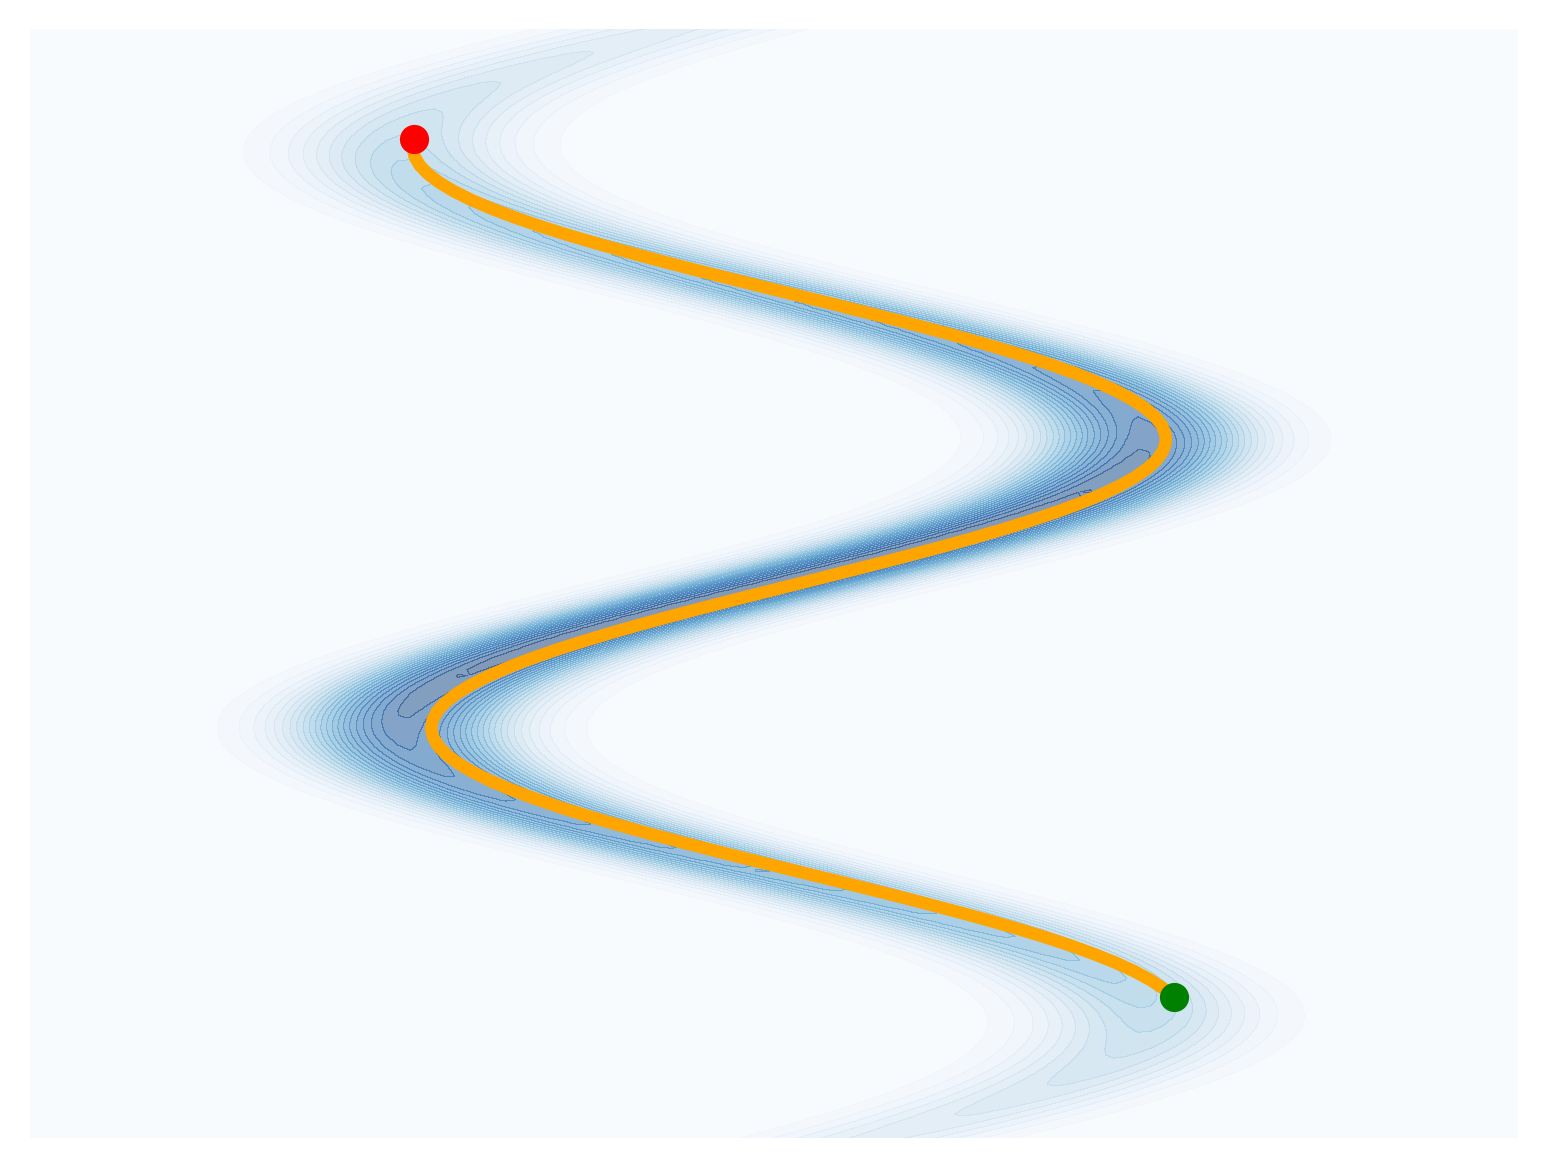
\includegraphics[width=\textwidth]{chapter5/results/visualisations/geodesics/gt.png}
        \caption{\scriptsize Ground Truth}
        \end{subfigure}
        \begin{subfigure}[b]{0.18\textwidth}
        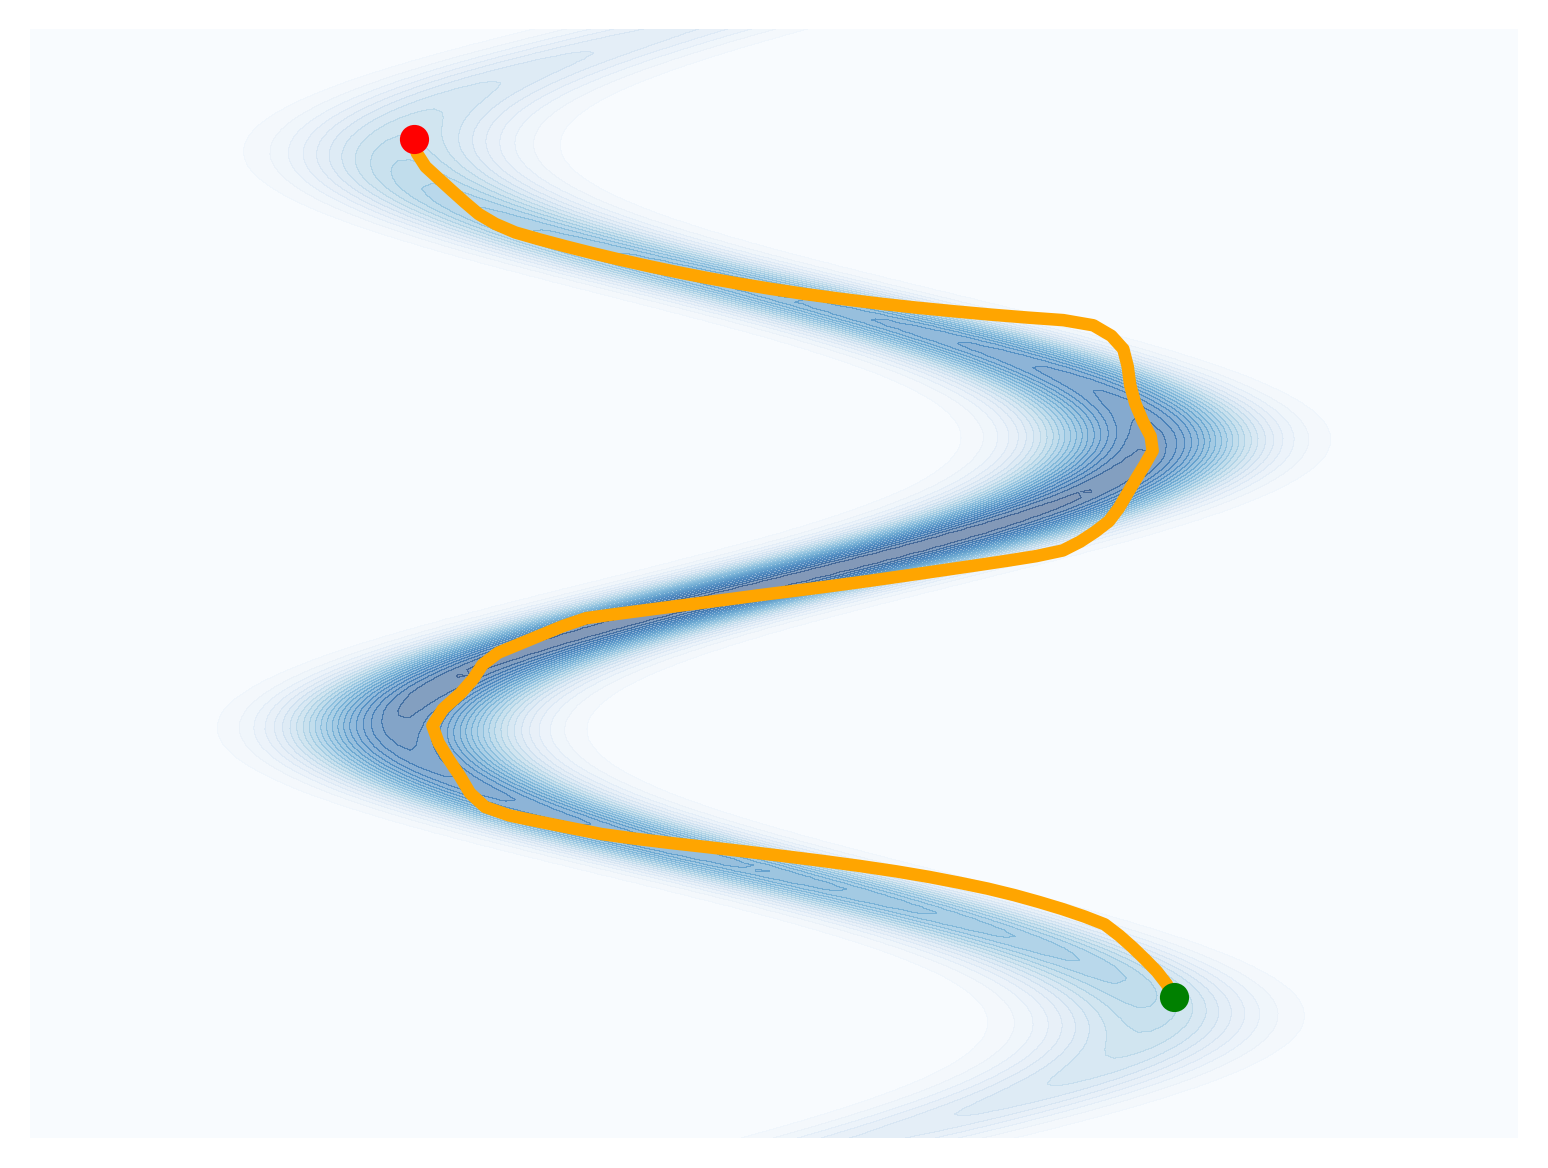
\includegraphics[width=\textwidth]{chapter5/results/visualisations/geodesics/ours.png}
        \caption{\scriptsize Our Method}
        \end{subfigure}
        \begin{subfigure}[b]{0.18\textwidth}
        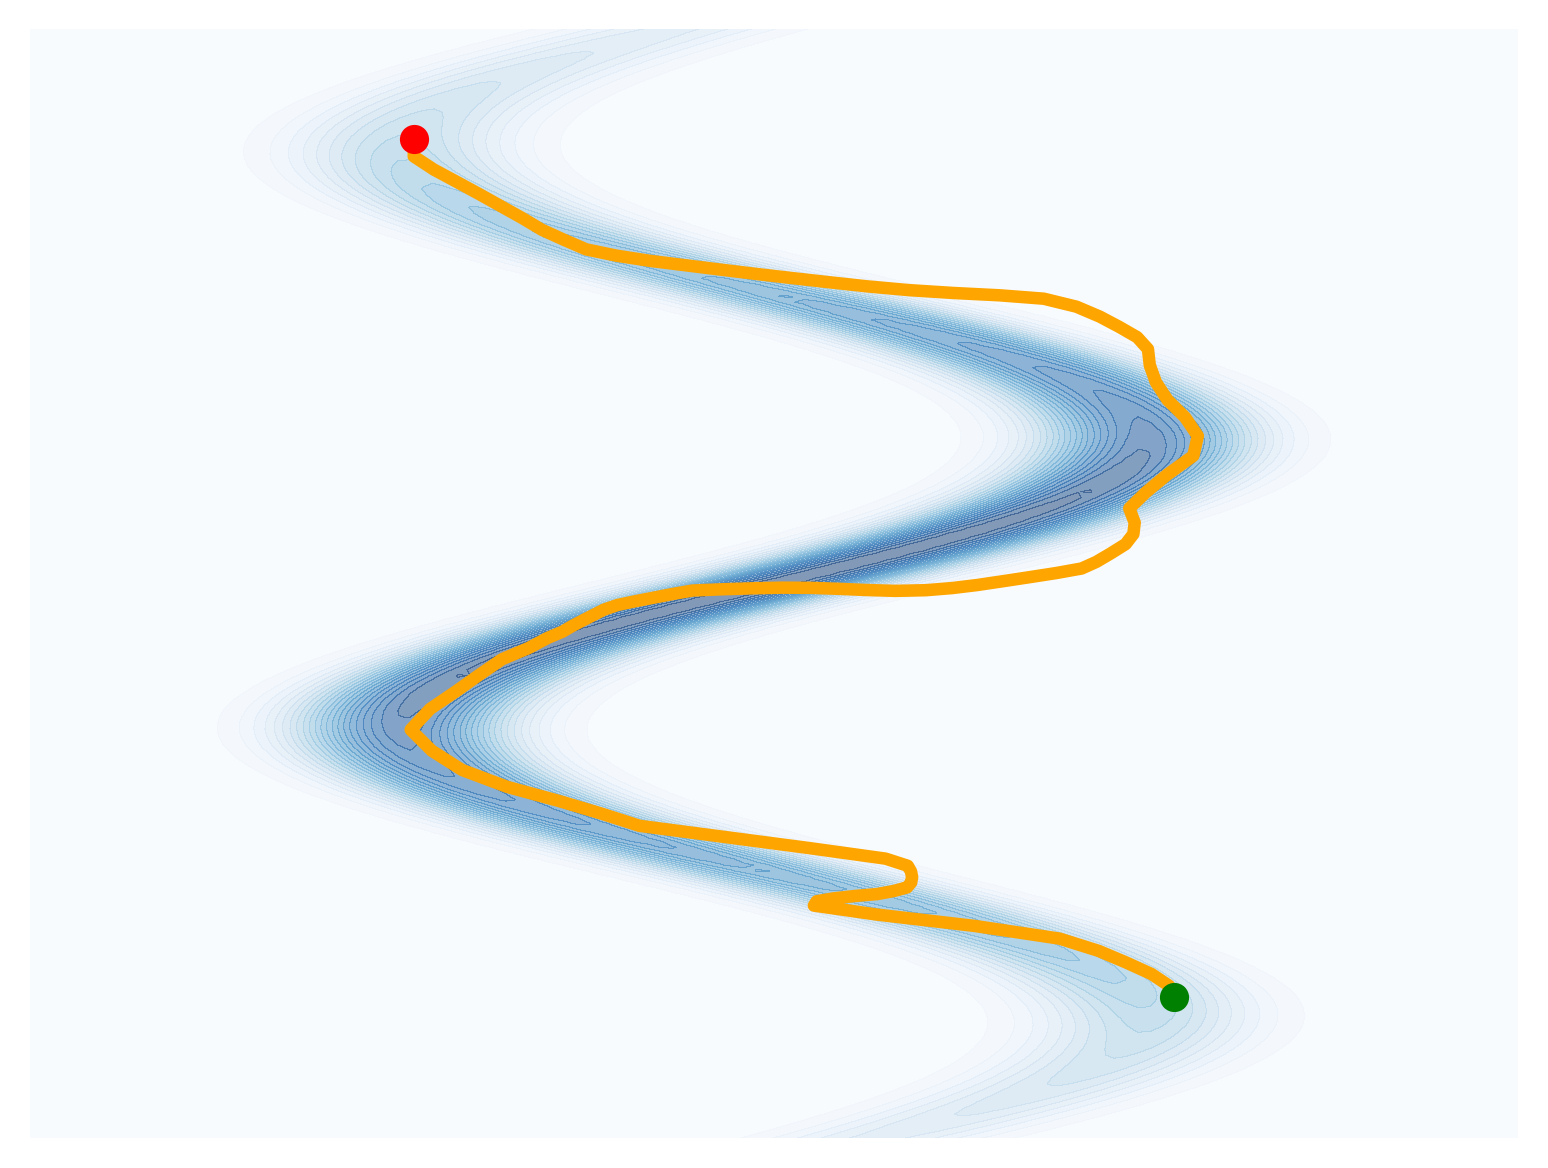
\includegraphics[width=\textwidth]{chapter5/results/visualisations/geodesics/standard_normal.png}
        \caption{\scriptsize Standard NF}
        \end{subfigure}
        \begin{subfigure}[b]{0.18\textwidth}
        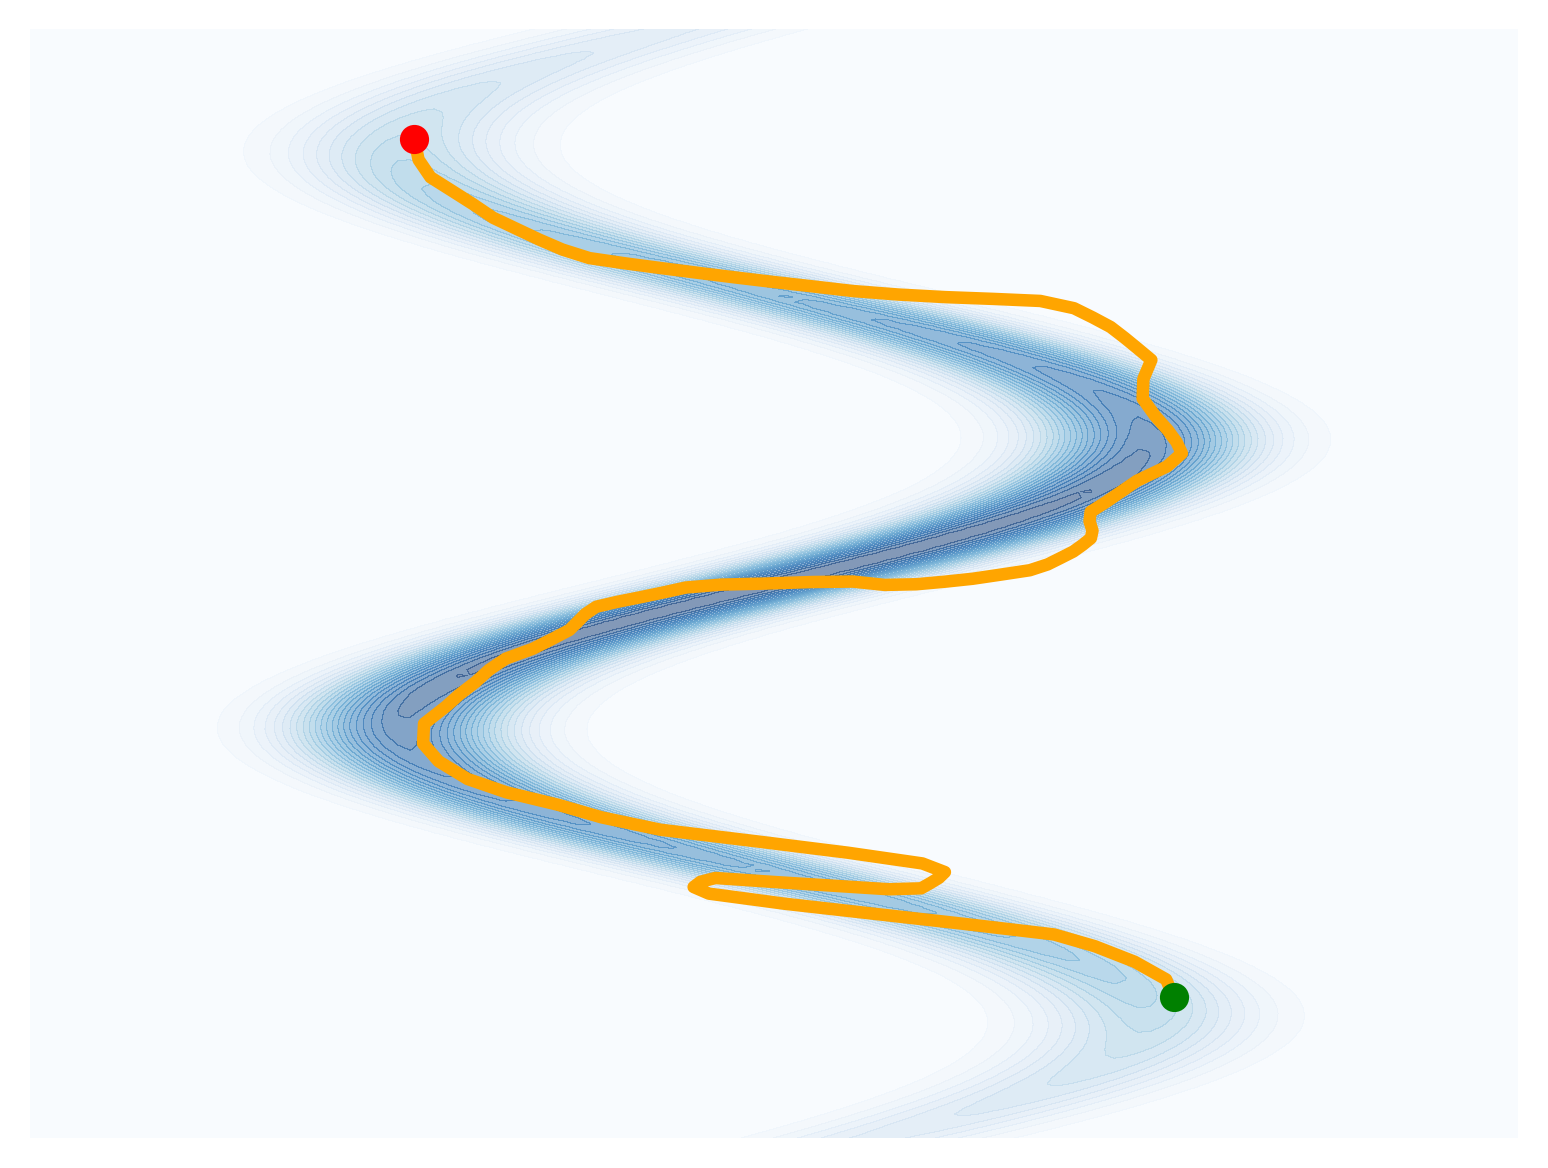
\includegraphics[width=\textwidth]{chapter5/results/visualisations/geodesics/standard_normal_anisotropic.png}
        \caption{\scriptsize Anisotropic NF}
        \end{subfigure}
        \begin{subfigure}[b]{0.18\textwidth}
        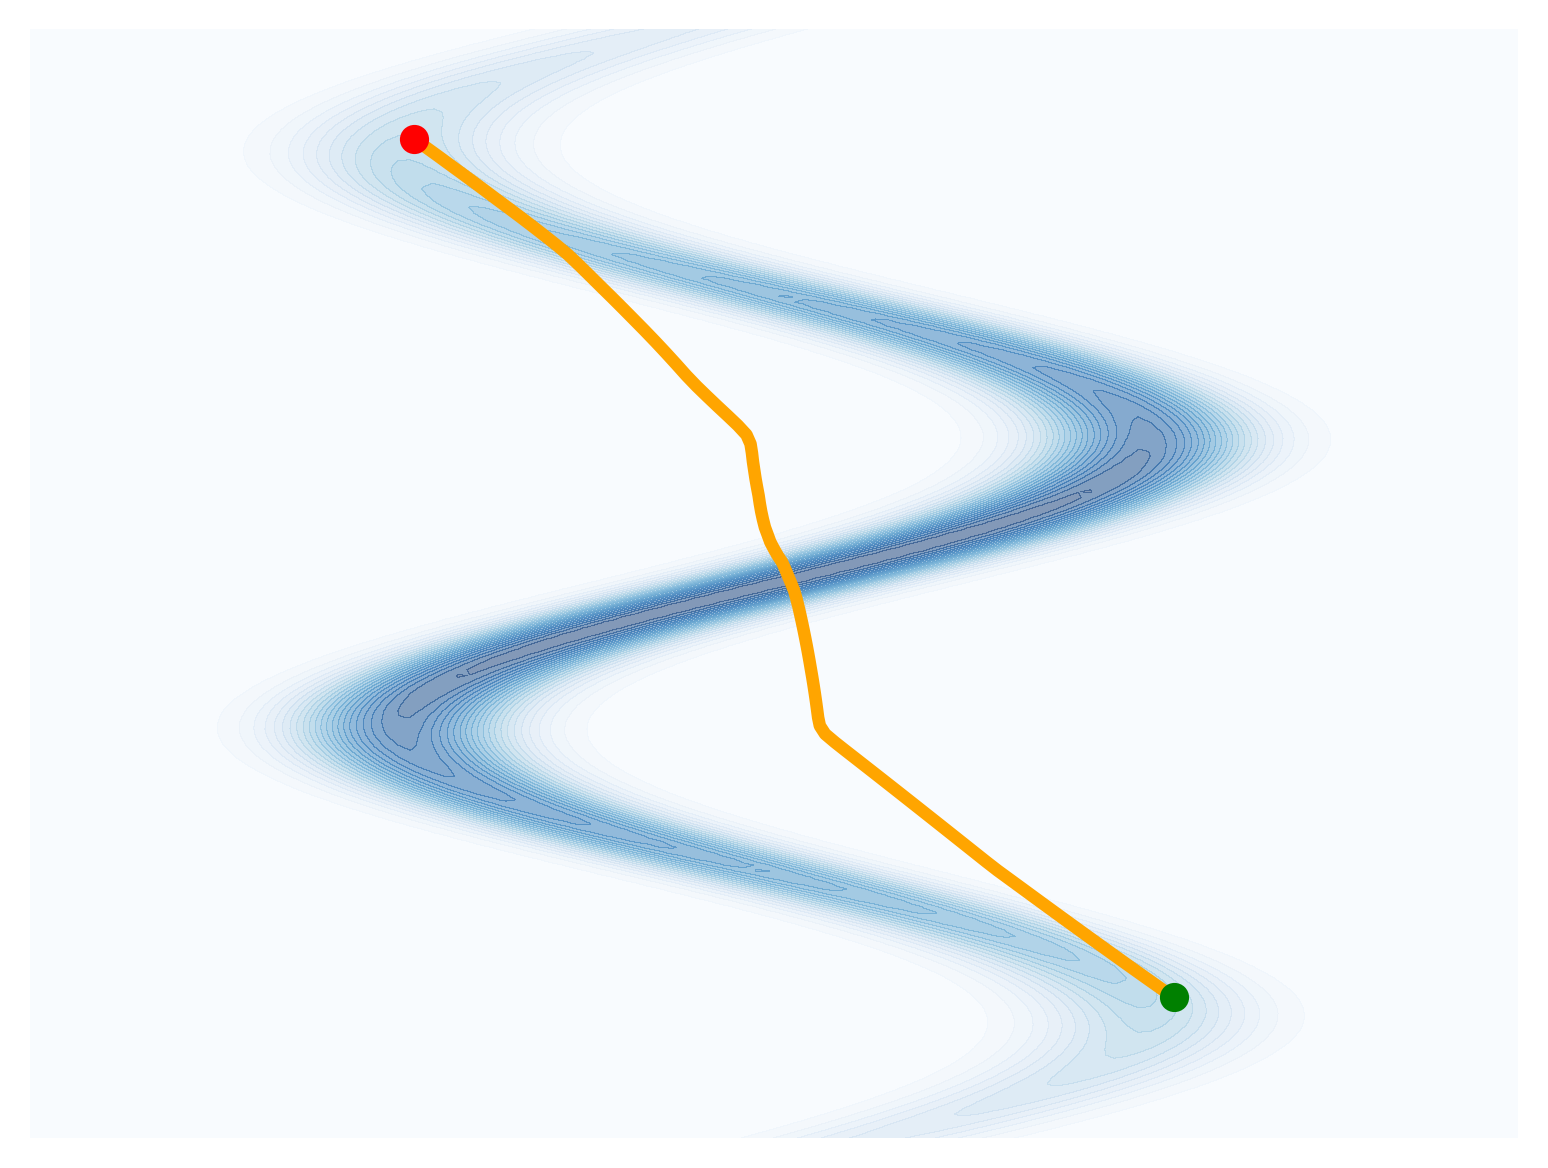
\includegraphics[width=\textwidth]{chapter5/results/visualisations/geodesics/isometricNF.png}
        \caption{\scriptsize Isometric NF}
        \end{subfigure}
        \caption{Comparison of geodesics computed using different methods on the river dataset. The geodesics generated by the proposed method have the fewest artifacts, aligning with expectations from Table~\ref{tab:geodesic-variation-errors}.}
        \label{fig:geodesics_comparison}
    \end{figure}
    

\subsection{Riemannian Autoencoder}\label{sec:RAE-experiments}
    
    To evaluate our method’s ability to learn a Riemannian autoencoder (RAE), we conducted experiments on both low-to-moderate dimensional \emph{Euclidean} datasets and higher-dimensional \emph{image} datasets:

    \begin{itemize}
        \item \textit{Hemisphere}($\dimInd'$, $\dimInd$) and \textit{Sinusoid}($\dimInd'$, $\dimInd$): Synthetic Euclidean datasets with controllable intrinsic dimension $\dimInd'$ and ambient dimension $\dimInd$.
        \item \(\dimInd'\)\emph{-Gaussian Blobs Image Manifold}: A synthetic image dataset, also with controllable intrinsic dimension $\dimInd'$, embedded in a 1024-dimensional ambient space.
        \item \textit{MNIST}: A dataset of handwritten digits, originally embedded in a 784-dimensional space, which we further embed into a 1024-dimensional ambient space using bicubic rescaling.
    \end{itemize}

    The \textit{Hemisphere} and \textit{Sinusoid} datasets are used to evaluate RAE's performance on low-to-moderate dimensional manifolds, while the \textit{Gaussian Blobs} and \textit{MNIST} datasets are used to test its scalability to higher-dimensional and more complex image manifolds. For further details on each dataset, refer to Appendix~\ref{app:rae_datasets}.


    \subsubsection{Euclidean datasets}
    \label{sec:euclidean_datasets}

    \paragraph{1D and 2D manifolds.}
    In Figures \ref{fig:learned_charts} and \ref{fig:rae_appendix_combined}, we present the data manifold approximations by our Riemannian autoencoder for four low-dimensional manifolds: Hemisphere(2,3), Sinusoid(1,3), Sinusoid(2,3) and Sinusoid(1,100). In Appendix~\ref{app:data_manifold_approximation}, we detail the process used to create the data manifold approximations for these experiments. In our experiments, we set \( \epsilon = 0.01 \), which resulted in \( d_{\epsilon} = \dimInd' \) for all cases, accurately capturing the intrinsic dimension of each manifold and producing accurate global charts.



    \paragraph{Higher-dimensional manifolds.}

    To assess the scalability of our method, we conducted experiments on the Hemisphere(5,20) and Sinusoid(5,20) datasets. The learned variances effectively indicate the importance of each latent dimension, with high variances corresponding to the intrinsic manifold structure. 

    On the Hemisphere(5,20) dataset, our model correctly identified five non-vanishing latent dimensions, achieving near-zero reconstruction error when selecting them. In contrast, choosing latent dimensions with vanishing variance resulted in no meaningful error reduction, confirming the model’s ability to separate important from redundant dimensions. A more detailed analysis of this effect is provided in Appendix~\ref{app:experimental-results}.

    For the more challenging Sinusoid(5,20) dataset, our method remains highly effective, though slightly less precise than for the Hemisphere dataset. The first six most important latent dimensions account for approximately $97\%$ of the variance, increasing to over $99\%$ with the seventh dimension. The model slightly overestimates the intrinsic dimensionality, likely due to the increased optimization challenges of learning a more intricate distribution while regularizing for isometry.

    \subsubsection{Image Datasets}\label{sec:image_datasets}


In our preliminary experiments on image datasets, we observed significant overestimation of the intrinsic dimension, despite the high quality of the geodesic interpolations. This issue stems from the use of non-affine flows,\footnote{We used compositions of affine coupling layers and $1 \times 1$ invertible convolutions, with the latter introducing non-affine transformations to the flow.} which increase the model’s flexibility but also inflate a Hessian-vector product term in the expansion of the Hessian of the model log-density. This inflation can disrupt the RAE’s ability to assign high variances to the most important latent dimensions (see Appendix~\ref{app:expanded_loss_function} for details).

To address this issue, we repeated the image experiments after including the Hessian vector product term as an additional regularization term in the loss function. The additional regularization term is given by:
\begin{align}
    \lambda_{\text{hess}} \, \mathbb{E}_{\stoVector \sim p_{\text{data}}}\Bigl[\bigl\|D^2_{\stoVector}\diffeo_{\networkParams_2} \cdot \spdMatrix_{\theta_1}^{-1} \diffeo_{\networkParams_2}(\stoVector)\bigr\|_2\Bigr],
\end{align}
where $\lambda_{\text{hess}}$ is the regularization weight, and $D^2_{\stoVector}\diffeo_{\networkParams_2}$ denotes the Hessian of the flow. As demonstrated in the following experiments, introducing this term substantially improved the RAE’s ability to correctly detect the intrinsic dimension while maintaining smooth geodesic paths and accurate reconstructions.

Computing the Hessian-vector product is impractical in high dimensions. To improve scalability, we instead minimize the norm of a single randomly chosen column of the Hessian-vector product (\(\mathbb{R}^{d \times d}\)) per iteration. This significantly reduces computational and memory overhead while preserving effectiveness. See Appendix~\ref{app:hvp-regularization} for details.
    
\begin{figure}[!htbp]
    \centering
    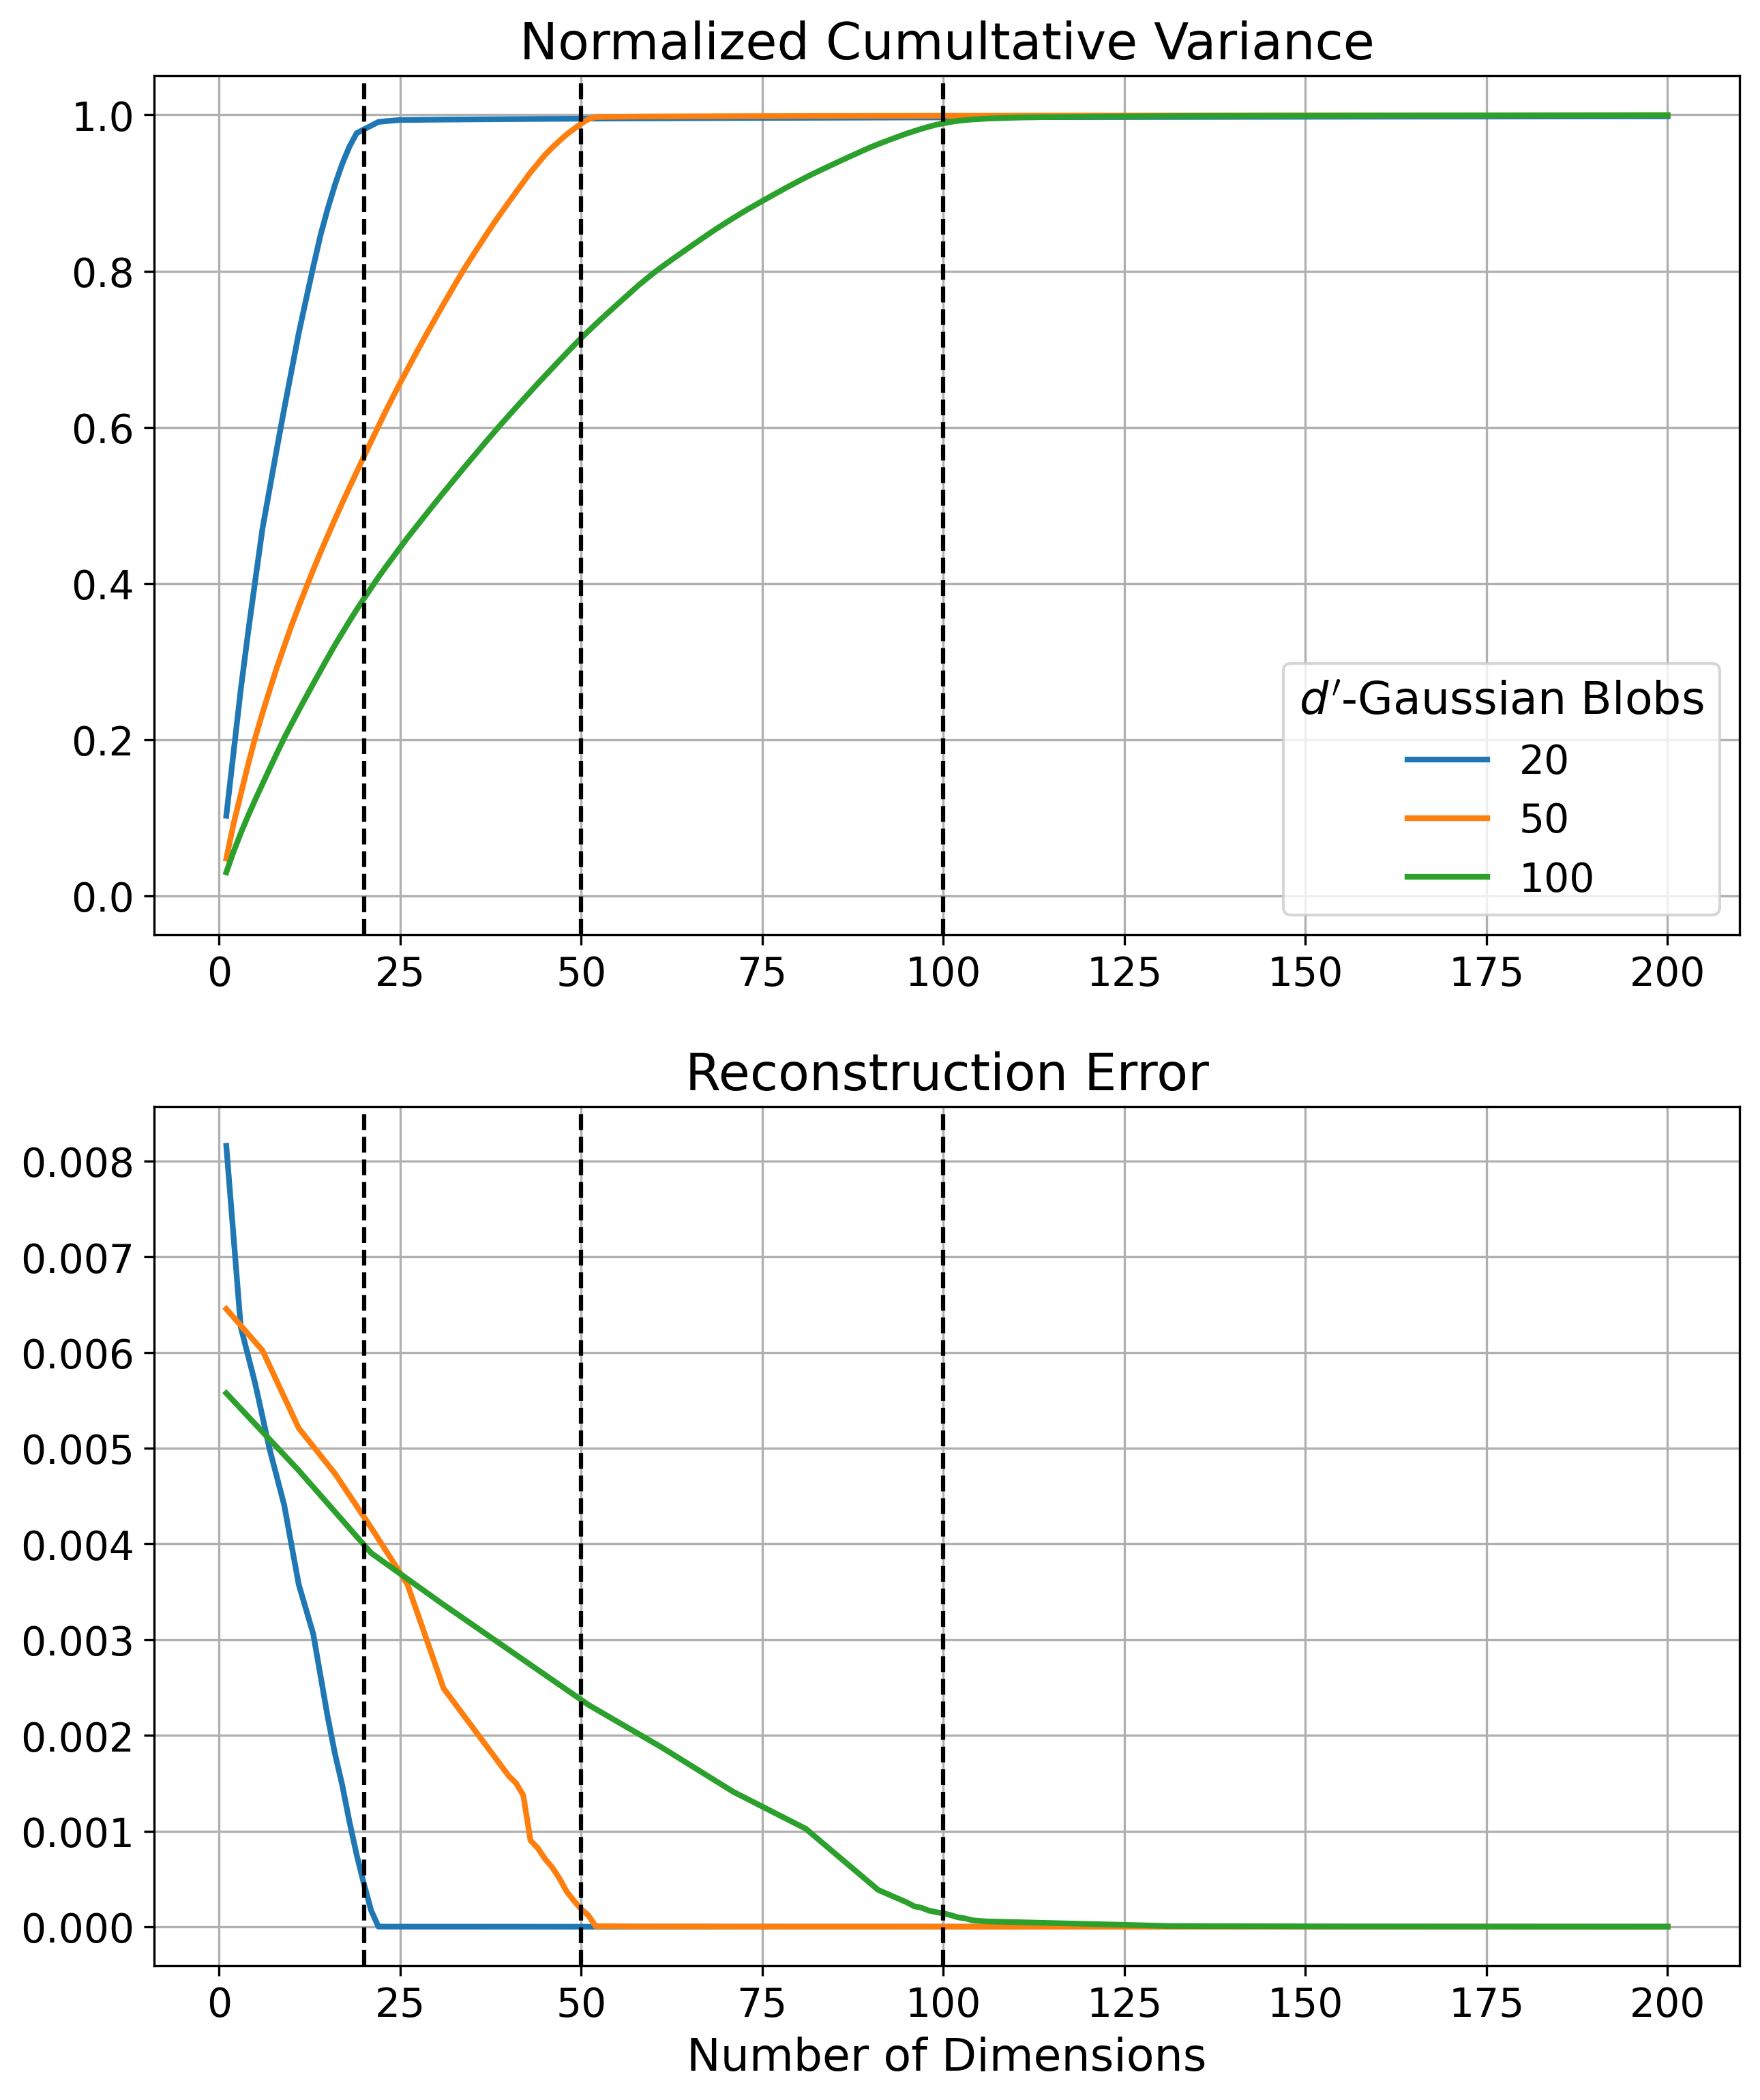
\includegraphics[width=\textwidth, height=0.6\textheight, keepaspectratio]{Chapter5/results/blobs/combined_variances_reconstruction_errors_plot.png}
    \caption{Normalized cumulative variance (top) and \(L^2\) reconstruction error (bottom) for \(d'\)-Gaussian Blobs with intrinsic dimensions \(d' = 20\), \(50\), and \(100\). Black dotted vertical lines mark the ground-truth intrinsic dimensions for each dataset. Curves are shown for the first 200 dimensions to highlight the critical range, as the behavior from 200 to 1024 dimensions remains effectively constant.}
    \label{fig:variance_reconstruction}
\end{figure}


\paragraph{\(d'\)-Gaussian Blobs.}
We evaluated our RAE on synthetic \emph{\(d'\)-Gaussian Blobs} manifolds embedded in a 1024-dimensional ambient space with intrinsic dimensions \(d' = 20\), \(50\), and \(100\). The RAE accurately captured the structure, assigning over 99\% of the total variance to 22, 51, and 101 latent dimensions respectively, closely aligning with the ground-truth intrinsic dimensions.

Figure~\ref{fig:variance_reconstruction} shows the normalized cumultative variance and the \(L^2\) reconstruction error as functions of the number of most important latent dimensions. All curves saturate very close to the ground truth intrinsic dimension demonstrating RAE’s ability to effectively capture the intrinsic structure of the data in high dimensional settings.


\paragraph{MNIST.}

\begin{figure}[!htbp]
    \centering
    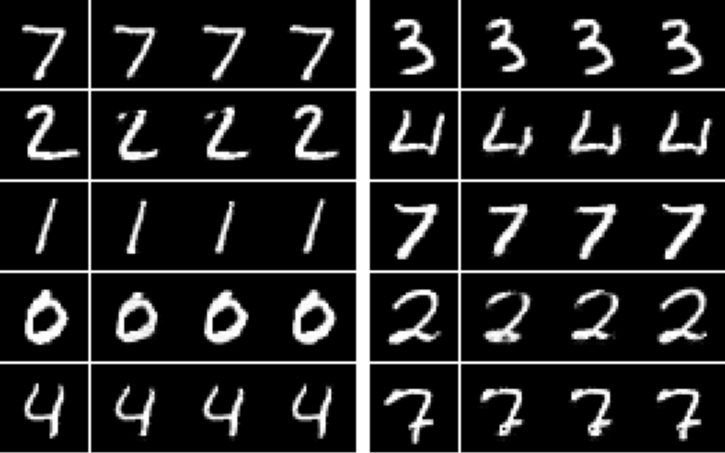
\includegraphics[width=\textwidth, height=0.33\textheight, keepaspectratio]{Chapter5/results/mnist/reconstruction.png}
        \caption{RAE reconstructions on MNIST. The leftmost column shows original images, while the next three show reconstructions for decreasing variance thresholds \(\epsilon\) (0.1, 0.05, 0.01), using 176, 208, and 271 latent dimensions, respectively. Reconstructions are clear at 176 dimensions and nearly indistinguishable from the originals at 271.}
    \label{fig:MNIST_reconstruction}
\end{figure}


We evaluated the RAE on the MNIST dataset, a real-world benchmark known for its multimodal distribution (each digit class represents a separate “mode”). While our method is theoretically best suited for unimodal distributions of the form in Equation~\ref{eq:stroco-diffeo-density}, it still performs remarkably well on MNIST, with only a slight tendency to overestimate the intrinsic dimension. Specifically, at \(\epsilon = 0.1\), the RAE assigns 90\% of the variance to 176 latent dimensions, which slightly exceeds the maximum local intrinsic dimension (LID) of 152 estimated by ID-DIFF, a state-of-the-art LID method \cite{pmlr-v235-stanczuk24a}.

We further examined two stricter variance thresholds, \(\epsilon = 0.05\) (208 dimensions) and \(\epsilon = 0.01\) (271 dimensions). Figure~\ref{fig:MNIST_reconstruction} shows that reconstructions are visually convincing at 176 dimensions and improve slightly with more dimensions, becoming nearly perfect at 271. We anticipate that incorporating more expressive transformations, such as rational quadratic spline flows \cite{durkan2019neural}, could further refine the dimensionality estimation and improve reconstruction quality by better handling the optimization challenges associated with learning the distribution under the isometry and Hessian constraints.
    
Overall, these experiments illustrate that our approach scales to real-world data, provided we incorporate the Hessian vector product regularization term when using non-affine flows. These results mark significant progress toward robust data-driven Riemannian geometry in high-dimensional settings.

    
\section{Conclusions}
\label{sec:conclusions}

In this work we have taken a first step towards a practical data-driven Riemannian geometry framework, striking a balance between scalability of training a data-driven Riemannian structure and of evaluating its corresponding manifold mappings. We have considered a family of unimodal probability densities whose negative log-likelihoods are compositions of strongly convex functions and diffeomorphisms, and sought to learn them. We have shown that once these unimodal densities are learned, the proposed score-based pullback geometry provides closed-form geodesics that pass through the data support and an interpretable Riemannian autoencoder with error bounds that estimates the intrinsic dimension of the data. Finally, to learn the distribution we have proposed an adaptation to normalizing flow training. Through numerical experiments on \textit{Euclidean} and \textit{image} datasets, we have shown that these modifications are crucial for extracting geometric information, and that our framework not only generates high-quality geodesics across the data support, but also accurately estimates the intrinsic dimension of the approximate data manifold while constructing a global chart, even in high-dimensional settings. 

Although the framework is theoretically best suited for unimodal distributions, it performs remarkably well on real multimodal distributions, albeit with a slight overestimation of intrinsic dimensionality. This highlights its practical utility for extracting geometry from real data. However, extending the formulation to better handle multimodal distributions remains an important direction for future work.

This work paves the way for scalable learning of data geometry, unlocking applications that were previously out of reach. It enables efficient computation of manifold maps such as geodesics and distances, with significant potential for advancing deep metric learning. Furthermore, it introduces Riemannian auto-encoders with interpretable latent spaces that effectively capture the intrinsic structure of data. Looking ahead, it paves the way for Riemannian optimization directly on the data manifold by enabling the computation of intrinsic gradients, with the potential to revolutionize inverse problem-solving and push the boundaries of controllable generative modeling.